% Options for packages loaded elsewhere
\PassOptionsToPackage{unicode}{hyperref}
\PassOptionsToPackage{hyphens}{url}
%
\documentclass[
]{article}
\title{ForecastCompetition}
\author{Ben and Yiyan}
\date{4/13/2022}

\usepackage{amsmath,amssymb}
\usepackage{lmodern}
\usepackage{iftex}
\ifPDFTeX
  \usepackage[T1]{fontenc}
  \usepackage[utf8]{inputenc}
  \usepackage{textcomp} % provide euro and other symbols
\else % if luatex or xetex
  \usepackage{unicode-math}
  \defaultfontfeatures{Scale=MatchLowercase}
  \defaultfontfeatures[\rmfamily]{Ligatures=TeX,Scale=1}
\fi
% Use upquote if available, for straight quotes in verbatim environments
\IfFileExists{upquote.sty}{\usepackage{upquote}}{}
\IfFileExists{microtype.sty}{% use microtype if available
  \usepackage[]{microtype}
  \UseMicrotypeSet[protrusion]{basicmath} % disable protrusion for tt fonts
}{}
\makeatletter
\@ifundefined{KOMAClassName}{% if non-KOMA class
  \IfFileExists{parskip.sty}{%
    \usepackage{parskip}
  }{% else
    \setlength{\parindent}{0pt}
    \setlength{\parskip}{6pt plus 2pt minus 1pt}}
}{% if KOMA class
  \KOMAoptions{parskip=half}}
\makeatother
\usepackage{xcolor}
\IfFileExists{xurl.sty}{\usepackage{xurl}}{} % add URL line breaks if available
\IfFileExists{bookmark.sty}{\usepackage{bookmark}}{\usepackage{hyperref}}
\hypersetup{
  pdftitle={ForecastCompetition},
  pdfauthor={Ben and Yiyan},
  hidelinks,
  pdfcreator={LaTeX via pandoc}}
\urlstyle{same} % disable monospaced font for URLs
\usepackage[margin=1in]{geometry}
\usepackage{color}
\usepackage{fancyvrb}
\newcommand{\VerbBar}{|}
\newcommand{\VERB}{\Verb[commandchars=\\\{\}]}
\DefineVerbatimEnvironment{Highlighting}{Verbatim}{commandchars=\\\{\}}
% Add ',fontsize=\small' for more characters per line
\usepackage{framed}
\definecolor{shadecolor}{RGB}{248,248,248}
\newenvironment{Shaded}{\begin{snugshade}}{\end{snugshade}}
\newcommand{\AlertTok}[1]{\textcolor[rgb]{0.94,0.16,0.16}{#1}}
\newcommand{\AnnotationTok}[1]{\textcolor[rgb]{0.56,0.35,0.01}{\textbf{\textit{#1}}}}
\newcommand{\AttributeTok}[1]{\textcolor[rgb]{0.77,0.63,0.00}{#1}}
\newcommand{\BaseNTok}[1]{\textcolor[rgb]{0.00,0.00,0.81}{#1}}
\newcommand{\BuiltInTok}[1]{#1}
\newcommand{\CharTok}[1]{\textcolor[rgb]{0.31,0.60,0.02}{#1}}
\newcommand{\CommentTok}[1]{\textcolor[rgb]{0.56,0.35,0.01}{\textit{#1}}}
\newcommand{\CommentVarTok}[1]{\textcolor[rgb]{0.56,0.35,0.01}{\textbf{\textit{#1}}}}
\newcommand{\ConstantTok}[1]{\textcolor[rgb]{0.00,0.00,0.00}{#1}}
\newcommand{\ControlFlowTok}[1]{\textcolor[rgb]{0.13,0.29,0.53}{\textbf{#1}}}
\newcommand{\DataTypeTok}[1]{\textcolor[rgb]{0.13,0.29,0.53}{#1}}
\newcommand{\DecValTok}[1]{\textcolor[rgb]{0.00,0.00,0.81}{#1}}
\newcommand{\DocumentationTok}[1]{\textcolor[rgb]{0.56,0.35,0.01}{\textbf{\textit{#1}}}}
\newcommand{\ErrorTok}[1]{\textcolor[rgb]{0.64,0.00,0.00}{\textbf{#1}}}
\newcommand{\ExtensionTok}[1]{#1}
\newcommand{\FloatTok}[1]{\textcolor[rgb]{0.00,0.00,0.81}{#1}}
\newcommand{\FunctionTok}[1]{\textcolor[rgb]{0.00,0.00,0.00}{#1}}
\newcommand{\ImportTok}[1]{#1}
\newcommand{\InformationTok}[1]{\textcolor[rgb]{0.56,0.35,0.01}{\textbf{\textit{#1}}}}
\newcommand{\KeywordTok}[1]{\textcolor[rgb]{0.13,0.29,0.53}{\textbf{#1}}}
\newcommand{\NormalTok}[1]{#1}
\newcommand{\OperatorTok}[1]{\textcolor[rgb]{0.81,0.36,0.00}{\textbf{#1}}}
\newcommand{\OtherTok}[1]{\textcolor[rgb]{0.56,0.35,0.01}{#1}}
\newcommand{\PreprocessorTok}[1]{\textcolor[rgb]{0.56,0.35,0.01}{\textit{#1}}}
\newcommand{\RegionMarkerTok}[1]{#1}
\newcommand{\SpecialCharTok}[1]{\textcolor[rgb]{0.00,0.00,0.00}{#1}}
\newcommand{\SpecialStringTok}[1]{\textcolor[rgb]{0.31,0.60,0.02}{#1}}
\newcommand{\StringTok}[1]{\textcolor[rgb]{0.31,0.60,0.02}{#1}}
\newcommand{\VariableTok}[1]{\textcolor[rgb]{0.00,0.00,0.00}{#1}}
\newcommand{\VerbatimStringTok}[1]{\textcolor[rgb]{0.31,0.60,0.02}{#1}}
\newcommand{\WarningTok}[1]{\textcolor[rgb]{0.56,0.35,0.01}{\textbf{\textit{#1}}}}
\usepackage{graphicx}
\makeatletter
\def\maxwidth{\ifdim\Gin@nat@width>\linewidth\linewidth\else\Gin@nat@width\fi}
\def\maxheight{\ifdim\Gin@nat@height>\textheight\textheight\else\Gin@nat@height\fi}
\makeatother
% Scale images if necessary, so that they will not overflow the page
% margins by default, and it is still possible to overwrite the defaults
% using explicit options in \includegraphics[width, height, ...]{}
\setkeys{Gin}{width=\maxwidth,height=\maxheight,keepaspectratio}
% Set default figure placement to htbp
\makeatletter
\def\fps@figure{htbp}
\makeatother
\setlength{\emergencystretch}{3em} % prevent overfull lines
\providecommand{\tightlist}{%
  \setlength{\itemsep}{0pt}\setlength{\parskip}{0pt}}
\setcounter{secnumdepth}{-\maxdimen} % remove section numbering
\usepackage{booktabs}
\usepackage{longtable}
\usepackage{array}
\usepackage{multirow}
\usepackage{wrapfig}
\usepackage{float}
\usepackage{colortbl}
\usepackage{pdflscape}
\usepackage{tabu}
\usepackage{threeparttable}
\usepackage{threeparttablex}
\usepackage[normalem]{ulem}
\usepackage{makecell}
\usepackage{xcolor}
\ifLuaTeX
  \usepackage{selnolig}  % disable illegal ligatures
\fi

\begin{document}
\maketitle

\hypertarget{data-cleaning}{%
\subsection{Data Cleaning}\label{data-cleaning}}

At this step, we cleaned the load, temperature, and humidity datasets.
First, we imported our datasets. Then we averaged the hourly temperature
and humidity across all weather stations. Then we cleaned these datasets
and hour hourly load data to return daily average temperature and
humidity across all weather stations. This process resulted in the
following three dataframes.

\begin{Shaded}
\begin{Highlighting}[]
\FunctionTok{library}\NormalTok{(readxl)}
\NormalTok{load }\OtherTok{\textless{}{-}} \FunctionTok{read\_excel}\NormalTok{(}\StringTok{"Data/load.xlsx"}\NormalTok{)}
\NormalTok{humidity }\OtherTok{\textless{}{-}} \FunctionTok{read\_excel}\NormalTok{(}\StringTok{"Data/relative\_humidity.xlsx"}\NormalTok{)}
\NormalTok{empty\_col2}\OtherTok{\textless{}{-}}\NormalTok{(}\StringTok{"humidity\_average"}\NormalTok{)}
\NormalTok{humidity[,empty\_col2]}\OtherTok{\textless{}{-}}\ConstantTok{NA}
\NormalTok{humidity}\SpecialCharTok{$}\NormalTok{humidity\_average}\OtherTok{\textless{}{-}}\FunctionTok{rowMeans}\NormalTok{(humidity[,(}\DecValTok{3}\SpecialCharTok{:}\DecValTok{30}\NormalTok{)])}
\NormalTok{temp }\OtherTok{\textless{}{-}} \FunctionTok{read\_excel}\NormalTok{(}\StringTok{"Data/temperature.xlsx"}\NormalTok{)}
\NormalTok{empty\_col3}\OtherTok{\textless{}{-}}\NormalTok{(}\StringTok{"temp\_average"}\NormalTok{)}
\NormalTok{temp[,empty\_col3]}\OtherTok{\textless{}{-}}\ConstantTok{NA}
\NormalTok{temp}\SpecialCharTok{$}\NormalTok{temp\_average}\OtherTok{\textless{}{-}}\FunctionTok{rowMeans}\NormalTok{(temp[,(}\DecValTok{3}\SpecialCharTok{:}\DecValTok{30}\NormalTok{)])}
\CommentTok{\#Separate the year, month, date using a pipe function}
\NormalTok{humidity\_2 }\OtherTok{\textless{}{-}}\NormalTok{ humidity }\SpecialCharTok{\%\textgreater{}\%} 
  \FunctionTok{mutate}\NormalTok{( }\AttributeTok{Date =} \FunctionTok{ymd}\NormalTok{(date)) }\SpecialCharTok{\%\textgreater{}\%} 
  \FunctionTok{mutate}\NormalTok{( }\AttributeTok{Year =} \FunctionTok{year}\NormalTok{(date), }
          \AttributeTok{Month =} \FunctionTok{month}\NormalTok{(date), }
          \AttributeTok{Day =} \FunctionTok{day}\NormalTok{(date)) }\SpecialCharTok{\%\textgreater{}\%} 
  \FunctionTok{select}\NormalTok{( Date, Year, Month, Day, humidity\_average)}
\NormalTok{temp\_2 }\OtherTok{\textless{}{-}}\NormalTok{ temp }\SpecialCharTok{\%\textgreater{}\%} 
  \FunctionTok{mutate}\NormalTok{( }\AttributeTok{Date =} \FunctionTok{ymd}\NormalTok{(date)) }\SpecialCharTok{\%\textgreater{}\%} 
  \FunctionTok{mutate}\NormalTok{( }\AttributeTok{Year =} \FunctionTok{year}\NormalTok{(date), }
          \AttributeTok{Month =} \FunctionTok{month}\NormalTok{(date), }
          \AttributeTok{Day =} \FunctionTok{day}\NormalTok{(date)) }\SpecialCharTok{\%\textgreater{}\%} 
  \FunctionTok{select}\NormalTok{( Date, Year, Month, Day, temp\_average)}
\CommentTok{\#Create a data frame with daily observations}
\NormalTok{humidity\_daily }\OtherTok{\textless{}{-}}\NormalTok{ humidity\_2 }\SpecialCharTok{\%\textgreater{}\%} 
  \FunctionTok{filter}\NormalTok{( }\SpecialCharTok{!}\FunctionTok{is.na}\NormalTok{(humidity\_average)) }\SpecialCharTok{\%\textgreater{}\%} 
  \FunctionTok{group\_by}\NormalTok{(Date,Year,Month,Day) }\SpecialCharTok{\%\textgreater{}\%} \CommentTok{\# here we left column with hour out to calculate daily mean}
  \FunctionTok{summarise}\NormalTok{( }\AttributeTok{daily\_humidity\_average =} \FunctionTok{mean}\NormalTok{(humidity\_average)) }
\NormalTok{temp\_daily }\OtherTok{\textless{}{-}}\NormalTok{ temp\_2 }\SpecialCharTok{\%\textgreater{}\%} 
  \FunctionTok{filter}\NormalTok{( }\SpecialCharTok{!}\FunctionTok{is.na}\NormalTok{(temp\_average)) }\SpecialCharTok{\%\textgreater{}\%} 
  \FunctionTok{group\_by}\NormalTok{(Date,Year,Month,Day) }\SpecialCharTok{\%\textgreater{}\%} \CommentTok{\# here we left column with hour out to calculate daily mean}
  \FunctionTok{summarise}\NormalTok{(}\AttributeTok{daily\_temp\_average =} \FunctionTok{mean}\NormalTok{(temp\_average))}
\CommentTok{\#Create an additional column for daily averages}
\NormalTok{empty\_col }\OtherTok{\textless{}{-}}\NormalTok{ (}\StringTok{"Daily Average"}\NormalTok{)}
\NormalTok{load[,empty\_col] }\OtherTok{\textless{}{-}} \ConstantTok{NA}
\NormalTok{load}\SpecialCharTok{$}\StringTok{\textasciigrave{}}\AttributeTok{Daily Average}\StringTok{\textasciigrave{}} \OtherTok{\textless{}{-}} \FunctionTok{rowMeans}\NormalTok{(load[,(}\DecValTok{3}\SpecialCharTok{:}\DecValTok{26}\NormalTok{)])}
\NormalTok{load }\OtherTok{\textless{}{-}}\NormalTok{ load[}\SpecialCharTok{{-}}\FunctionTok{c}\NormalTok{(}\DecValTok{1}\NormalTok{,}\DecValTok{3}\SpecialCharTok{:}\DecValTok{26}\NormalTok{)]}
\NormalTok{temp\_daily}\OtherTok{\textless{}{-}}\NormalTok{temp\_daily[,}\SpecialCharTok{{-}}\FunctionTok{c}\NormalTok{(}\DecValTok{2}\SpecialCharTok{:}\DecValTok{4}\NormalTok{)]}
\NormalTok{humidity\_daily}\OtherTok{\textless{}{-}}\NormalTok{humidity\_daily[,}\SpecialCharTok{{-}}\FunctionTok{c}\NormalTok{(}\DecValTok{2}\SpecialCharTok{:}\DecValTok{4}\NormalTok{)]}
\CommentTok{\#Display output}
\FunctionTok{head}\NormalTok{(load, }\DecValTok{10}\NormalTok{)}
\end{Highlighting}
\end{Shaded}

\begin{verbatim}
## # A tibble: 10 x 2
##    date                `Daily Average`
##    <dttm>                        <dbl>
##  1 2005-01-01 00:00:00           2889.
##  2 2005-01-02 00:00:00           2789.
##  3 2005-01-03 00:00:00           2708.
##  4 2005-01-04 00:00:00           2212.
##  5 2005-01-05 00:00:00           2035.
##  6 2005-01-06 00:00:00           2110.
##  7 2005-01-07 00:00:00           2313.
##  8 2005-01-08 00:00:00           2480.
##  9 2005-01-09 00:00:00           3116.
## 10 2005-01-10 00:00:00           3222.
\end{verbatim}

\begin{Shaded}
\begin{Highlighting}[]
\FunctionTok{head}\NormalTok{(temp\_daily, }\DecValTok{10}\NormalTok{)}
\end{Highlighting}
\end{Shaded}

\begin{verbatim}
## # A tibble: 10 x 2
## # Groups:   Date [10]
##    Date       daily_temp_average
##    <date>                  <dbl>
##  1 2005-01-01               53.6
##  2 2005-01-02               53.8
##  3 2005-01-03               55.9
##  4 2005-01-04               61.7
##  5 2005-01-05               60.4
##  6 2005-01-06               62.0
##  7 2005-01-07               55.9
##  8 2005-01-08               57.7
##  9 2005-01-09               47.6
## 10 2005-01-10               49.3
\end{verbatim}

\begin{Shaded}
\begin{Highlighting}[]
\FunctionTok{head}\NormalTok{(humidity\_daily, }\DecValTok{10}\NormalTok{)}
\end{Highlighting}
\end{Shaded}

\begin{verbatim}
## # A tibble: 10 x 2
## # Groups:   Date [10]
##    Date       daily_humidity_average
##    <date>                      <dbl>
##  1 2005-01-01                   76.7
##  2 2005-01-02                   80.5
##  3 2005-01-03                   81.2
##  4 2005-01-04                   74.8
##  5 2005-01-05                   76.1
##  6 2005-01-06                   78.0
##  7 2005-01-07                   71.7
##  8 2005-01-08                   81.8
##  9 2005-01-09                   72.7
## 10 2005-01-10                   81.1
\end{verbatim}

\hypertarget{create-ts-object-and-create-test-and-training-data}{%
\subsection{Create ts object and create test and training
data}\label{create-ts-object-and-create-test-and-training-data}}

At this step, we create time-series projects for load, temp, and
humidity, with weekly and yearly seasonality. The original data are from
2005 to 2010. Then, we created a training (2005-2009) and a testing
(Jan, 2010) dataset for each of the three variables. We also decomposed
the load data and created the deseasonal load data.

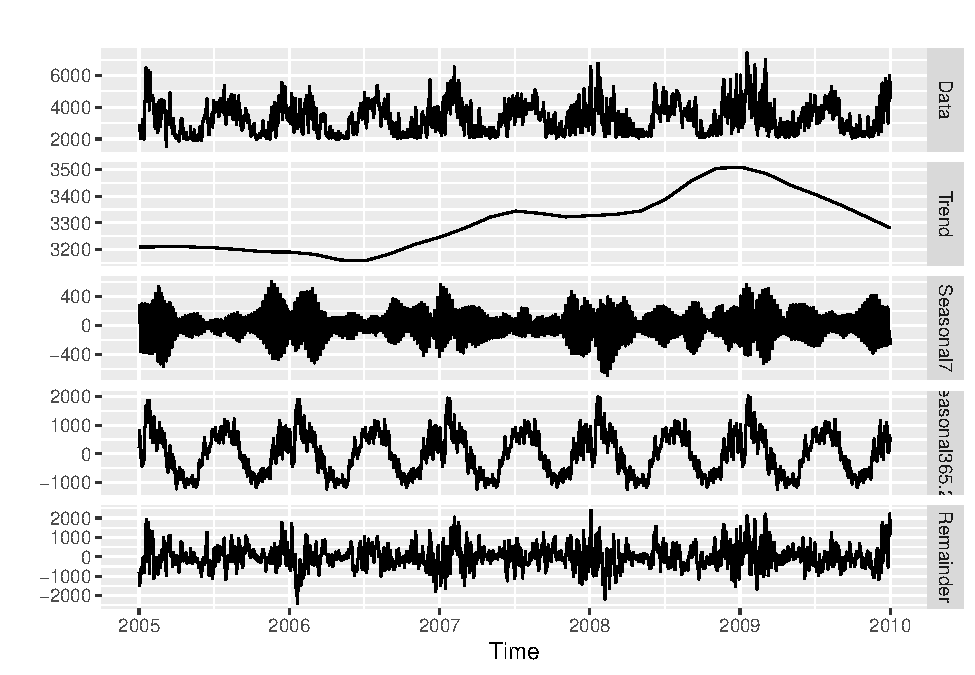
\includegraphics{ForecastCompetition_vFinal_files/figure-latex/pressure-1.pdf}
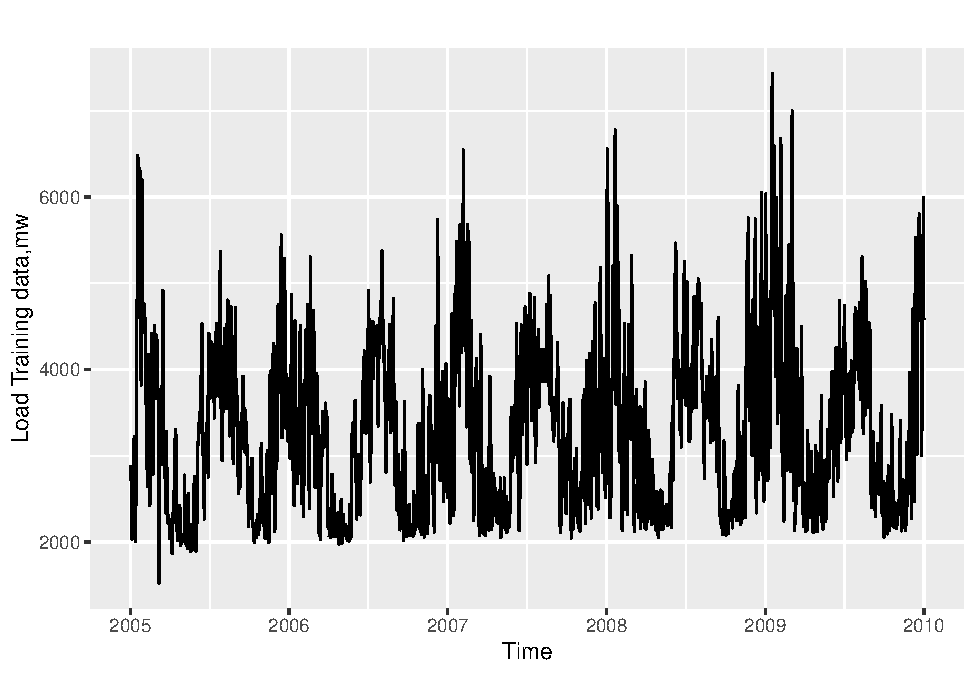
\includegraphics{ForecastCompetition_vFinal_files/figure-latex/pressure-2.pdf}
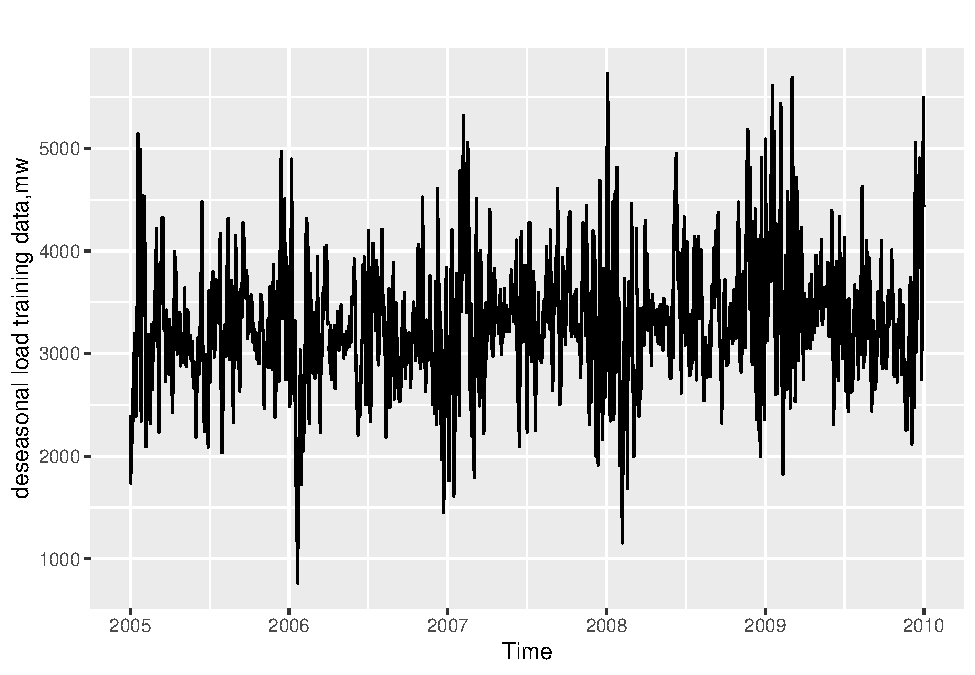
\includegraphics{ForecastCompetition_vFinal_files/figure-latex/pressure-3.pdf}

\#\#4 Simple models At this step, we applied 4 simple models to the load
training data to generate forecasts for Jan 2010. The 4 models are
arithmetic mean on original data, arithmetic mean on deseasonal data,
seasonal naïve on original data, and naïve on deseasonal data. Because
these forecasting methods are very basic, they do not have very high
accuracy.

\begin{Shaded}
\begin{Highlighting}[]
\CommentTok{\#Arithmetic mean on original data}
\NormalTok{MEAN\_seas }\OtherTok{\textless{}{-}} \FunctionTok{meanf}\NormalTok{(}\AttributeTok{y =}\NormalTok{ ts\_load\_09, }\AttributeTok{h =} \DecValTok{31}\NormalTok{)}
\FunctionTok{autoplot}\NormalTok{(MEAN\_seas)}\SpecialCharTok{+}\FunctionTok{ylab}\NormalTok{(}\StringTok{"Mean\_seas, mw"}\NormalTok{)}
\end{Highlighting}
\end{Shaded}

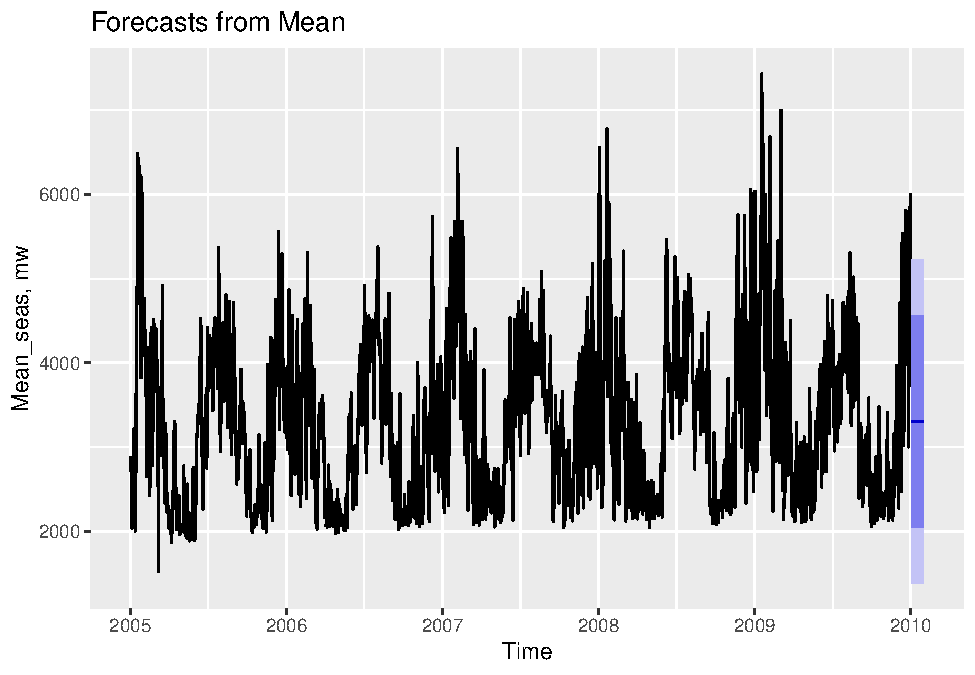
\includegraphics{ForecastCompetition_vFinal_files/figure-latex/unnamed-chunk-1-1.pdf}

\begin{Shaded}
\begin{Highlighting}[]
\CommentTok{\#Arithmetic mean on deseas data}
\NormalTok{MEAN\_deseas }\OtherTok{\textless{}{-}} \FunctionTok{meanf}\NormalTok{(deseasonal\_load\_09, }\AttributeTok{h=}\DecValTok{31}\NormalTok{)}
\FunctionTok{autoplot}\NormalTok{(MEAN\_deseas)}\SpecialCharTok{+}\FunctionTok{ylab}\NormalTok{(}\StringTok{"MEAN\_deseas,mw"}\NormalTok{)}
\end{Highlighting}
\end{Shaded}

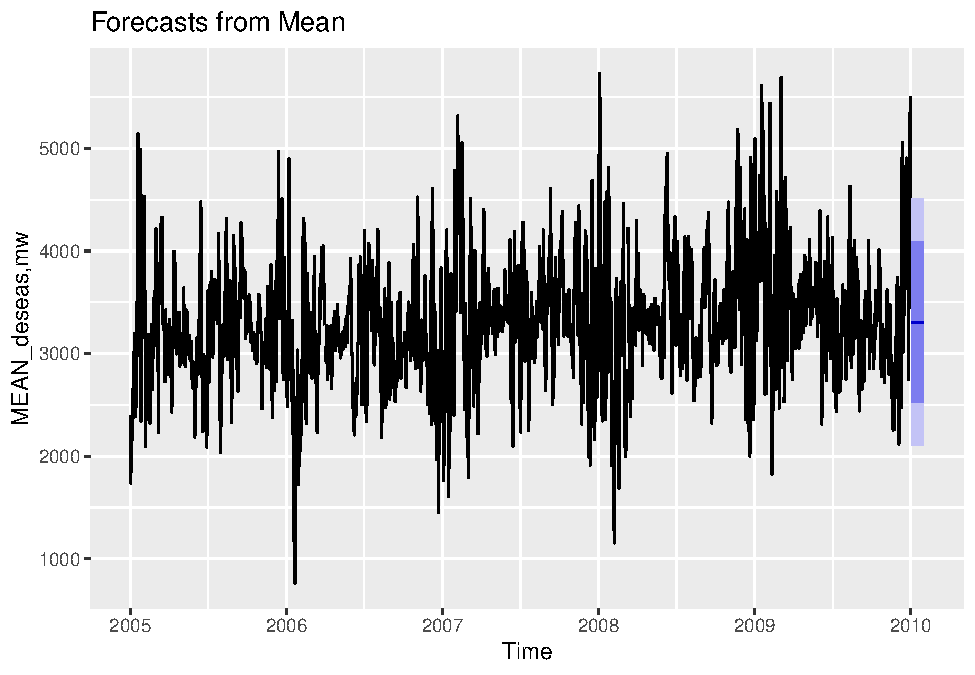
\includegraphics{ForecastCompetition_vFinal_files/figure-latex/unnamed-chunk-1-2.pdf}

\begin{Shaded}
\begin{Highlighting}[]
\CommentTok{\#Seasonal naive on original data}
\NormalTok{SNAIVE\_seas }\OtherTok{\textless{}{-}} \FunctionTok{snaive}\NormalTok{(ts\_load\_09, }\AttributeTok{h=}\DecValTok{31}\NormalTok{)}
\FunctionTok{autoplot}\NormalTok{(SNAIVE\_seas)}\SpecialCharTok{+}\FunctionTok{ylab}\NormalTok{(}\StringTok{"SNAIVE\_seas,mw"}\NormalTok{)}
\end{Highlighting}
\end{Shaded}

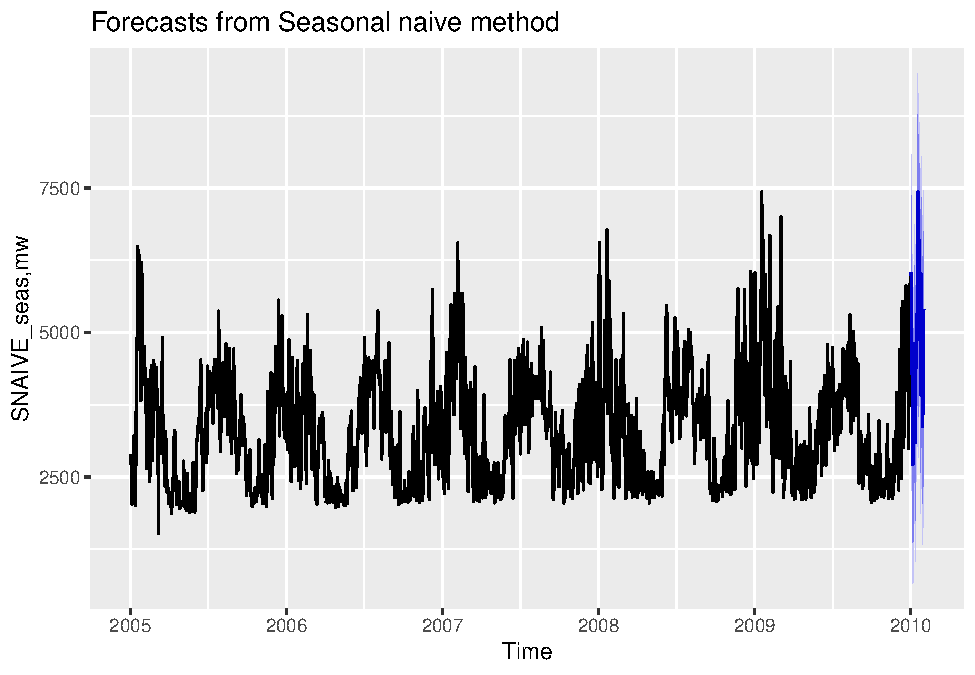
\includegraphics{ForecastCompetition_vFinal_files/figure-latex/unnamed-chunk-1-3.pdf}

\begin{Shaded}
\begin{Highlighting}[]
\CommentTok{\#Naive on deseas data}
\NormalTok{NAIVE\_deseas }\OtherTok{\textless{}{-}} \FunctionTok{naive}\NormalTok{(deseasonal\_load\_09, }\AttributeTok{h=}\DecValTok{31}\NormalTok{)}
\FunctionTok{autoplot}\NormalTok{(NAIVE\_deseas)}\SpecialCharTok{+}\FunctionTok{ylab}\NormalTok{(}\StringTok{"NAIVE\_deseas,mw"}\NormalTok{)}
\end{Highlighting}
\end{Shaded}

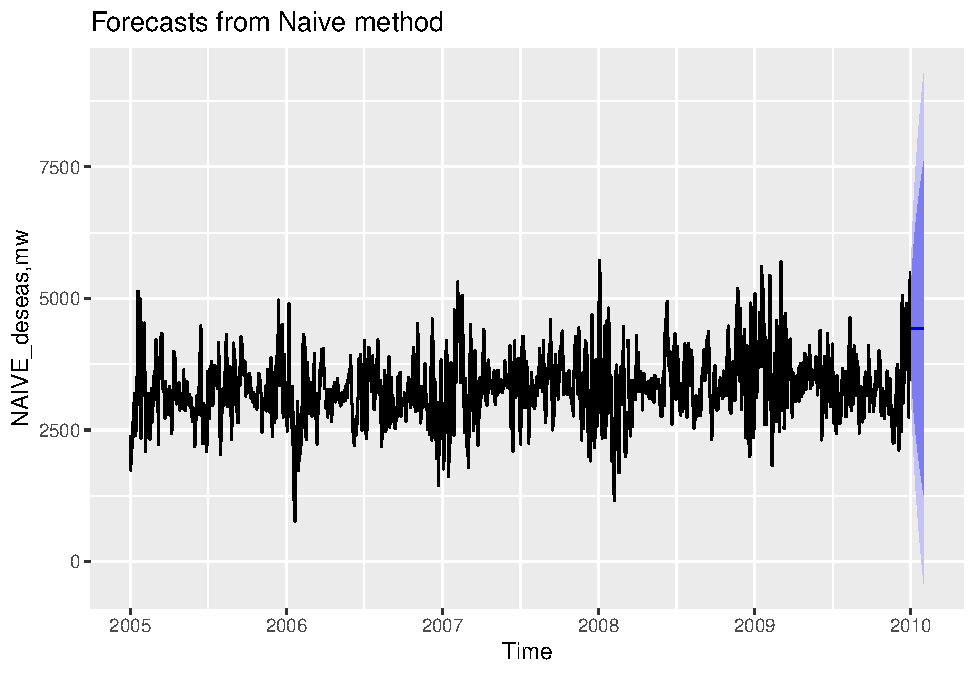
\includegraphics{ForecastCompetition_vFinal_files/figure-latex/unnamed-chunk-1-4.pdf}
\#\#Manually explore ARIMA At this step, we first ran the ADF test, the
p-value is less than 0.01, implying that there is no unit root. Then, we
ran the seasonal Mann-Kendall test, 2-sided p-value =8.6608e-12,
implying that there is a trend in the series. To manually explore ARIMA
model, we first ran the n\_diff function, differenced the series
accordingly, and created ACF and PACF for the differenced data. When
looking at the first 12 lags for ACF and PACF, we see the ACF shows a
slow decay and PACF shows a cutoff at lag 4. Indicating p=4,q=0, and we
know that d=1. There are no significant lags at 12, 24\ldots{} in ACF
and PACF, thus it has no seasonal components in the seasonal ARIMA
model. The model we used is (4,1,0)(0,0,0). The output is a forecast
using this model.

\begin{Shaded}
\begin{Highlighting}[]
\DocumentationTok{\#\#adf test}
\NormalTok{deseasonal\_load\_09 }\OtherTok{\textless{}{-}} \FunctionTok{na.fill}\NormalTok{(deseasonal\_load\_09,}\StringTok{"extend"}\NormalTok{)}
\FunctionTok{adf.test}\NormalTok{(deseasonal\_load\_09,}\AttributeTok{alternative=}\StringTok{"stationary"}\NormalTok{)}
\end{Highlighting}
\end{Shaded}

\begin{verbatim}
## 
##  Augmented Dickey-Fuller Test
## 
## data:  deseasonal_load_09
## Dickey-Fuller = -11.298, Lag order = 12, p-value = 0.01
## alternative hypothesis: stationary
\end{verbatim}

\begin{Shaded}
\begin{Highlighting}[]
\DocumentationTok{\#\#seasonal Mann{-}Kendall test}
\FunctionTok{SeasonalMannKendall}\NormalTok{(deseasonal\_load\_09)}
\end{Highlighting}
\end{Shaded}

\begin{verbatim}
## tau = 0.146, 2-sided pvalue =8.6608e-12
\end{verbatim}

\begin{Shaded}
\begin{Highlighting}[]
\CommentTok{\#Use n\_diff to find out the number of differencing needed}
\NormalTok{n\_diff\_trend }\OtherTok{\textless{}{-}} \FunctionTok{ndiffs}\NormalTok{(deseasonal\_load\_09)}
\FunctionTok{cat}\NormalTok{(}\StringTok{"Number of differencing needed: "}\NormalTok{,n\_diff\_trend)}
\end{Highlighting}
\end{Shaded}

\begin{verbatim}
## Number of differencing needed:  1
\end{verbatim}

\begin{Shaded}
\begin{Highlighting}[]
\DocumentationTok{\#\#d=1}
\NormalTok{ns\_diff\_seasonal }\OtherTok{\textless{}{-}} \FunctionTok{nsdiffs}\NormalTok{(ts\_load\_09)}
\FunctionTok{cat}\NormalTok{(}\StringTok{"Number of seasonal differencing needed: "}\NormalTok{,ns\_diff\_seasonal)}
\end{Highlighting}
\end{Shaded}

\begin{verbatim}
## Number of seasonal differencing needed:  0
\end{verbatim}

\begin{Shaded}
\begin{Highlighting}[]
\DocumentationTok{\#\#D=0}
\NormalTok{ts\_load\_09\_diff }\OtherTok{\textless{}{-}} \FunctionTok{diff}\NormalTok{(ts\_load\_09,}\AttributeTok{lag =}\DecValTok{1}\NormalTok{, }\AttributeTok{differences=}\DecValTok{1}\NormalTok{) }
\DocumentationTok{\#\#Create ACF and PACF}
\FunctionTok{par}\NormalTok{(}\AttributeTok{mfrow=}\FunctionTok{c}\NormalTok{(}\DecValTok{1}\NormalTok{,}\DecValTok{2}\NormalTok{))}
\FunctionTok{Acf}\NormalTok{(ts\_load\_09\_diff,}\AttributeTok{lag.max=}\DecValTok{60}\NormalTok{,}\AttributeTok{main=}\StringTok{"Differenced Load"}\NormalTok{,}\AttributeTok{ylim=}\FunctionTok{c}\NormalTok{(}\SpecialCharTok{{-}}\DecValTok{1}\NormalTok{,}\DecValTok{1}\NormalTok{))}
\FunctionTok{Pacf}\NormalTok{(ts\_load\_09\_diff,}\AttributeTok{lag.max=}\DecValTok{60}\NormalTok{,}\AttributeTok{main=}\StringTok{"Differenced Load"}\NormalTok{,}\AttributeTok{ylim=}\FunctionTok{c}\NormalTok{(}\SpecialCharTok{{-}}\DecValTok{1}\NormalTok{,}\DecValTok{1}\NormalTok{))}
\end{Highlighting}
\end{Shaded}

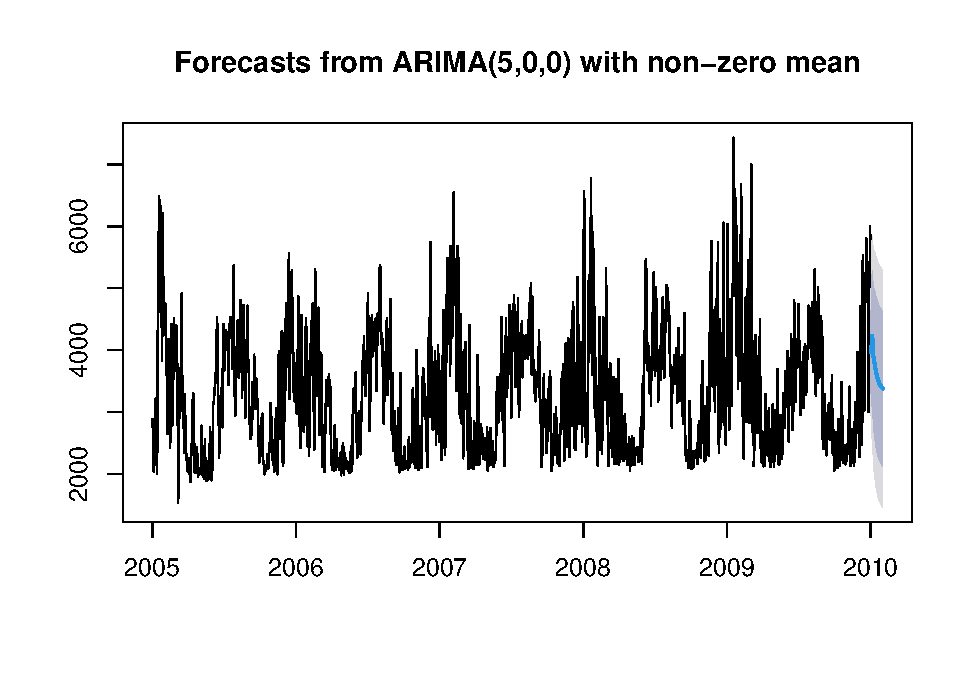
\includegraphics{ForecastCompetition_vFinal_files/figure-latex/unnamed-chunk-2-1.pdf}

\begin{Shaded}
\begin{Highlighting}[]
\DocumentationTok{\#\#Forecast using manual sarima model }
\NormalTok{SARIMA\_Model }\OtherTok{\textless{}{-}} \FunctionTok{Arima}\NormalTok{(ts\_load\_09,}\AttributeTok{order=}\FunctionTok{c}\NormalTok{(}\DecValTok{4}\NormalTok{,}\DecValTok{1}\NormalTok{,}\DecValTok{0}\NormalTok{),}\AttributeTok{seasonal=}\FunctionTok{c}\NormalTok{(}\DecValTok{0}\NormalTok{,}\DecValTok{0}\NormalTok{,}\DecValTok{0}\NormalTok{),}\AttributeTok{include.drift=}\ConstantTok{FALSE}\NormalTok{)}
\FunctionTok{print}\NormalTok{(SARIMA\_Model)}
\end{Highlighting}
\end{Shaded}

\begin{verbatim}
## Series: ts_load_09 
## ARIMA(4,1,0) 
## 
## Coefficients:
##          ar1      ar2      ar3      ar4
##       0.0503  -0.3465  -0.1037  -0.1741
## s.e.  0.0232   0.0230   0.0230   0.0231
## 
## sigma^2 = 273250:  log likelihood = -13974.3
## AIC=27958.6   AICc=27958.64   BIC=27986.15
\end{verbatim}

\begin{Shaded}
\begin{Highlighting}[]
\NormalTok{SARIMA\_forecast}\OtherTok{\textless{}{-}}\NormalTok{forecast}\SpecialCharTok{::}\FunctionTok{forecast}\NormalTok{(}\AttributeTok{object=}\NormalTok{SARIMA\_Model,}\AttributeTok{h=}\DecValTok{31}\NormalTok{)}
\FunctionTok{autoplot}\NormalTok{(SARIMA\_forecast)}\SpecialCharTok{+}\FunctionTok{ylab}\NormalTok{(}\StringTok{"maually created SARIMA\_forecast,mw"}\NormalTok{)}
\end{Highlighting}
\end{Shaded}

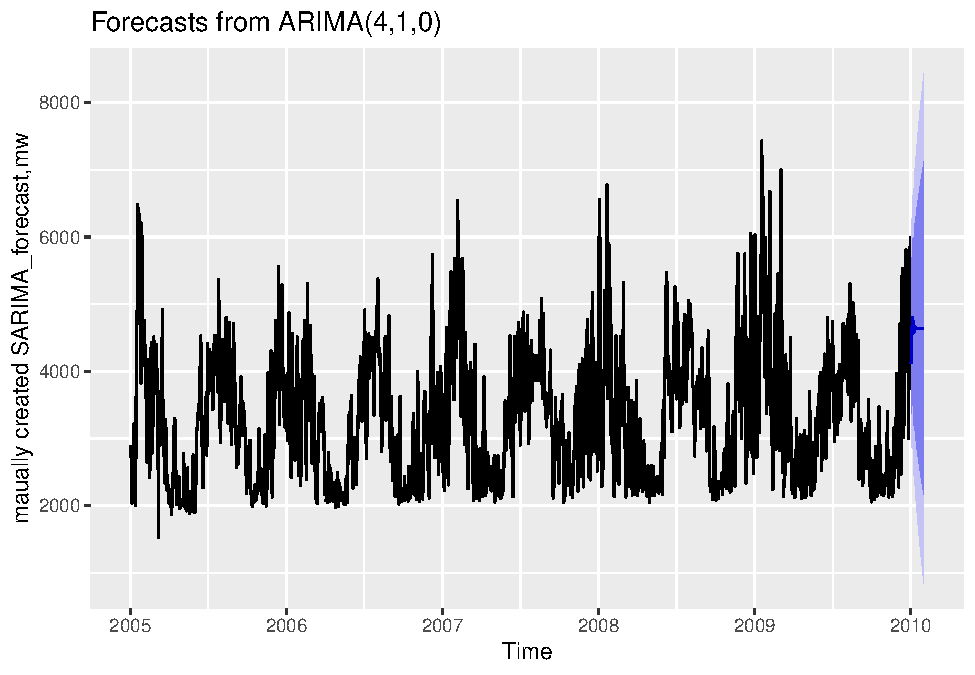
\includegraphics{ForecastCompetition_vFinal_files/figure-latex/unnamed-chunk-2-2.pdf}

\#\#Auto ARIMA We ran the auto ARIMA function on our time series load
data. We ran A Seasonal ARIMA model on the original load data, obtaining
a model of ARIMA (5,0,0) and no seasonal component. The AIC score is
27905.49. we also ran an ARIMA model on the deseasonal data, obtaining a
model of ARIMA (1,1,1) and an AIC of 27334.23. Surprisingly, the order
of the non-seasonal components between the two models is quite
different. Because these two models ran on two different series, their
AICs are not directly comparable.

\begin{Shaded}
\begin{Highlighting}[]
\CommentTok{\# Model:  SARIMA on original data}
\NormalTok{SARIMA\_autofit }\OtherTok{\textless{}{-}} \FunctionTok{auto.arima}\NormalTok{(ts\_load\_09)}
\FunctionTok{print}\NormalTok{(SARIMA\_autofit)}
\end{Highlighting}
\end{Shaded}

\begin{verbatim}
## Series: ts_load_09 
## ARIMA(5,0,0) with non-zero mean 
## 
## Coefficients:
##          ar1      ar2     ar3      ar4     ar5      mean
##       1.0045  -0.3993  0.2156  -0.0727  0.1272  3306.509
## s.e.  0.0233   0.0331  0.0340   0.0331  0.0233    95.523
## 
## sigma^2 = 262752:  log likelihood = -13945.75
## AIC=27905.49   AICc=27905.55   BIC=27944.06
\end{verbatim}

\begin{Shaded}
\begin{Highlighting}[]
\NormalTok{SARIMA\_forecast }\OtherTok{\textless{}{-}}\NormalTok{ forecast}\SpecialCharTok{::}\FunctionTok{forecast}\NormalTok{(}\AttributeTok{object =}\NormalTok{ SARIMA\_autofit, }\AttributeTok{h =} \DecValTok{31}\NormalTok{)}
\FunctionTok{plot}\NormalTok{(SARIMA\_forecast)}
\end{Highlighting}
\end{Shaded}

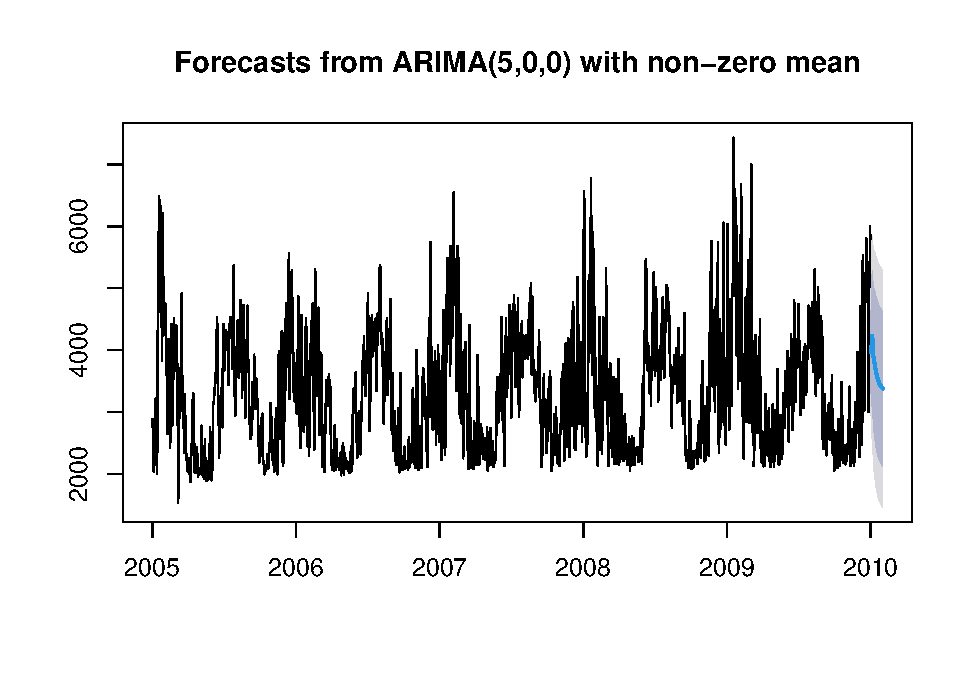
\includegraphics{ForecastCompetition_vFinal_files/figure-latex/unnamed-chunk-3-1.pdf}

\begin{Shaded}
\begin{Highlighting}[]
\CommentTok{\# Model:  ARIMA on deseasonal data}
\NormalTok{ARIMA\_autofit }\OtherTok{\textless{}{-}} \FunctionTok{auto.arima}\NormalTok{(deseasonal\_load\_09, }\AttributeTok{max.D =} \DecValTok{0}\NormalTok{, }\AttributeTok{max.P =} \DecValTok{0}\NormalTok{, }\AttributeTok{max.Q =} \DecValTok{0}\NormalTok{)}
\FunctionTok{print}\NormalTok{(ARIMA\_autofit)}
\end{Highlighting}
\end{Shaded}

\begin{verbatim}
## Series: deseasonal_load_09 
## ARIMA(1,1,1) with drift 
## 
## Coefficients:
##           ar1     ma1    drift
##       -0.3881  0.5913   1.0916
## s.e.   0.0541  0.0449  11.5834
## 
## sigma^2 = 186653:  log likelihood = -13663.11
## AIC=27334.23   AICc=27334.25   BIC=27356.27
\end{verbatim}

\begin{Shaded}
\begin{Highlighting}[]
\NormalTok{ARIMA\_forecast }\OtherTok{\textless{}{-}}\NormalTok{ forecast}\SpecialCharTok{::}\FunctionTok{forecast}\NormalTok{(}\AttributeTok{object =}\NormalTok{ ARIMA\_autofit, }\AttributeTok{h =} \DecValTok{31}\NormalTok{)}
\FunctionTok{plot}\NormalTok{(ARIMA\_forecast)}
\end{Highlighting}
\end{Shaded}

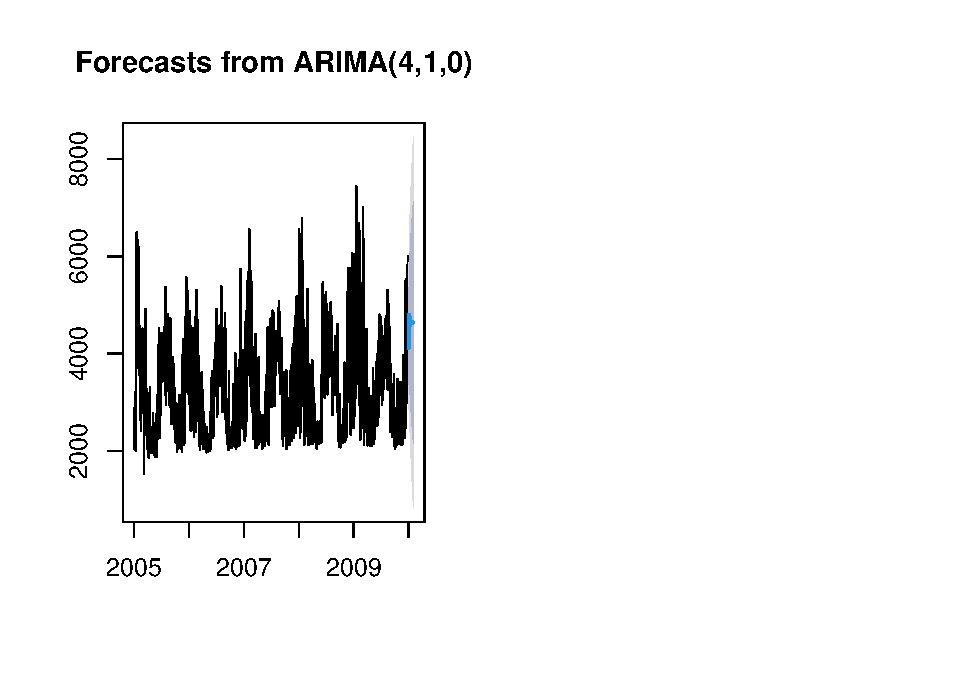
\includegraphics{ForecastCompetition_vFinal_files/figure-latex/unnamed-chunk-3-2.pdf}
\#\#ARIMA + FOURIER terms In this section, we ran an ARIMA model with
fourier terms and an ARIMA model with fourier terms and the exogenous
regressors. We first created a matrix with the fourier terms and a
matrix with fouier terms and the exogenous variables. The training
period is used to fit the ARIMA model and the testing period is used to
forecast the ARIMA model. Lastly, we plotted the forecast results and
compared them with the observed data.

\begin{Shaded}
\begin{Highlighting}[]
\DocumentationTok{\#\#Create a matrix of just the fourier terms and a matrix with the fourier terms and the exogenous regressors. }
\NormalTok{fourier\_mat}\OtherTok{\textless{}{-}}\FunctionTok{fourier}\NormalTok{(ts\_load\_09,}\AttributeTok{K=}\FunctionTok{c}\NormalTok{(}\DecValTok{2}\NormalTok{,}\DecValTok{12}\NormalTok{),}\AttributeTok{h=}\FunctionTok{nrow}\NormalTok{(ts\_load\_09))}
\NormalTok{fourier\_mat\_for}\OtherTok{\textless{}{-}}\FunctionTok{fourier}\NormalTok{(ts\_load\_09,}\AttributeTok{K=}\FunctionTok{c}\NormalTok{(}\DecValTok{2}\NormalTok{,}\DecValTok{12}\NormalTok{),}\AttributeTok{h=}\DecValTok{31}\NormalTok{)}
\NormalTok{xregs\_fourier}\OtherTok{\textless{}{-}}\FunctionTok{cbind}\NormalTok{(fourier\_mat,xregs\_train)}
\NormalTok{xregs\_for}\OtherTok{\textless{}{-}}\NormalTok{xregs\_daily[(}\FunctionTok{nrow}\NormalTok{(xregs\_fourier)}\SpecialCharTok{+}\DecValTok{1}\NormalTok{)}\SpecialCharTok{:}\NormalTok{(}\FunctionTok{nrow}\NormalTok{(xregs\_fourier)}\SpecialCharTok{+}\DecValTok{31}\NormalTok{),]}
\NormalTok{xregs\_fourier\_for}\OtherTok{\textless{}{-}}\FunctionTok{cbind}\NormalTok{(fourier\_mat\_for,xregs\_for)}


\NormalTok{ts\_load\_compare}\OtherTok{\textless{}{-}}\FunctionTok{subset}\NormalTok{(ts\_load,}\AttributeTok{end=}\FunctionTok{length}\NormalTok{(ts\_load\_09)}\SpecialCharTok{+}\DecValTok{31}\NormalTok{)}

\DocumentationTok{\#\#without exogenous regressors}
\DocumentationTok{\#\#Fit ARIMA with fourier matrix}
\NormalTok{ARIMA\_Four\_fit }\OtherTok{\textless{}{-}} \FunctionTok{auto.arima}\NormalTok{(ts\_load\_09, }
                             \AttributeTok{seasonal=}\ConstantTok{FALSE}\NormalTok{, }
                             \AttributeTok{lambda=}\DecValTok{0}\NormalTok{,}
                             \AttributeTok{xreg=}\NormalTok{fourier\_mat}
\NormalTok{                             )}
\CommentTok{\#Forecast with ARIMA fit}
\NormalTok{ARIMA\_Four\_for }\OtherTok{\textless{}{-}}\NormalTok{ forecast}\SpecialCharTok{::}\FunctionTok{forecast}\NormalTok{(ARIMA\_Four\_fit,}
                           \AttributeTok{xreg=}\NormalTok{fourier\_mat\_for,}
                           \AttributeTok{h=}\DecValTok{31}
\NormalTok{                           ) }
\CommentTok{\#Plot foresting results}
\FunctionTok{autoplot}\NormalTok{(ARIMA\_Four\_for) }\SpecialCharTok{+} \FunctionTok{ylab}\NormalTok{(}\StringTok{"Load"}\NormalTok{)}
\end{Highlighting}
\end{Shaded}

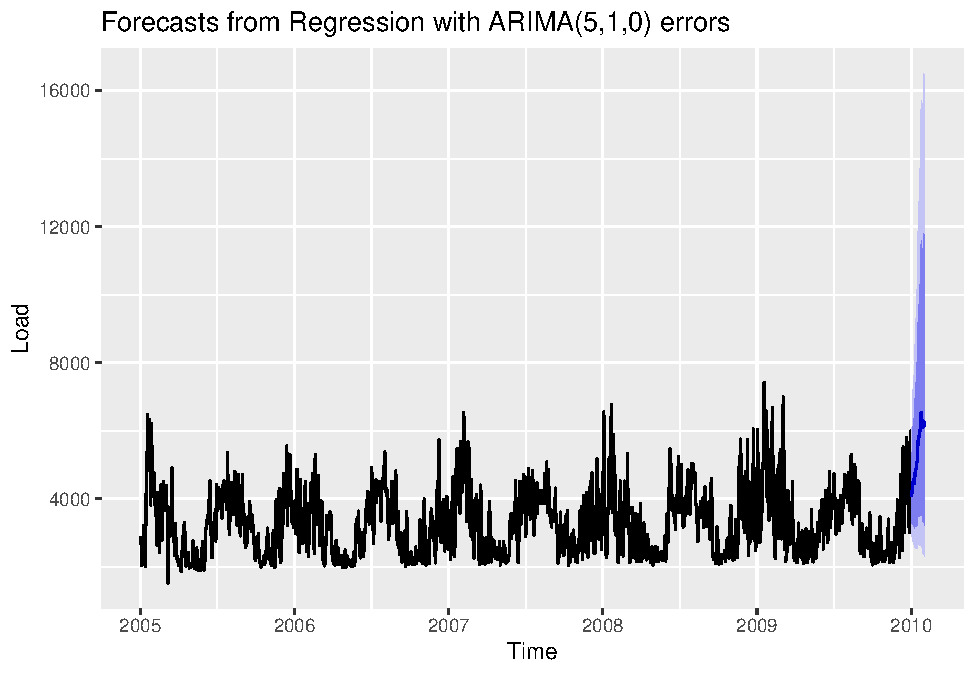
\includegraphics{ForecastCompetition_vFinal_files/figure-latex/unnamed-chunk-4-1.pdf}

\begin{Shaded}
\begin{Highlighting}[]
\CommentTok{\#Plot model + observed data}
\FunctionTok{autoplot}\NormalTok{(ts\_load) }\SpecialCharTok{+}
  \FunctionTok{autolayer}\NormalTok{(ARIMA\_Four\_for, }\AttributeTok{series=}\StringTok{"ARIMA\_FOURIER"}\NormalTok{,}\AttributeTok{PI=}\ConstantTok{FALSE}\NormalTok{) }\SpecialCharTok{+}
  \FunctionTok{ylab}\NormalTok{(}\StringTok{"Load"}\NormalTok{)}
\end{Highlighting}
\end{Shaded}

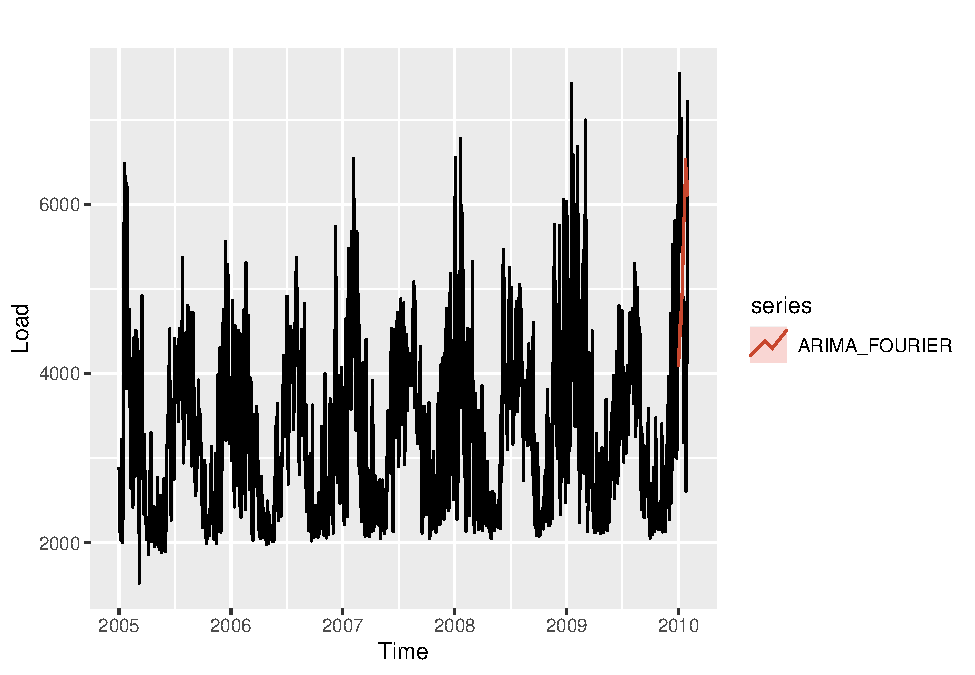
\includegraphics{ForecastCompetition_vFinal_files/figure-latex/unnamed-chunk-4-2.pdf}

\begin{Shaded}
\begin{Highlighting}[]
\DocumentationTok{\#\#with exogenous regressors }
\NormalTok{ARIMA\_Four\_fit2 }\OtherTok{\textless{}{-}} \FunctionTok{auto.arima}\NormalTok{(ts\_load\_09, }
                             \AttributeTok{seasonal=}\ConstantTok{FALSE}\NormalTok{, }
                             \AttributeTok{lambda=}\DecValTok{0}\NormalTok{,}
                             \AttributeTok{xreg=}\NormalTok{xregs\_fourier}
\NormalTok{                             )}
\CommentTok{\#Forecast with ARIMA fit}
\NormalTok{ARIMA\_Four\_for2 }\OtherTok{\textless{}{-}}\NormalTok{ forecast}\SpecialCharTok{::}\FunctionTok{forecast}\NormalTok{(ARIMA\_Four\_fit2,}
                                     \AttributeTok{xreg=}\NormalTok{xregs\_fourier\_for,}
                           \AttributeTok{h=}\DecValTok{31}
\NormalTok{                           ) }
\CommentTok{\#Plot foresting results}
\FunctionTok{autoplot}\NormalTok{(ARIMA\_Four\_for2) }\SpecialCharTok{+} \FunctionTok{ylab}\NormalTok{(}\StringTok{"Load"}\NormalTok{)}
\end{Highlighting}
\end{Shaded}

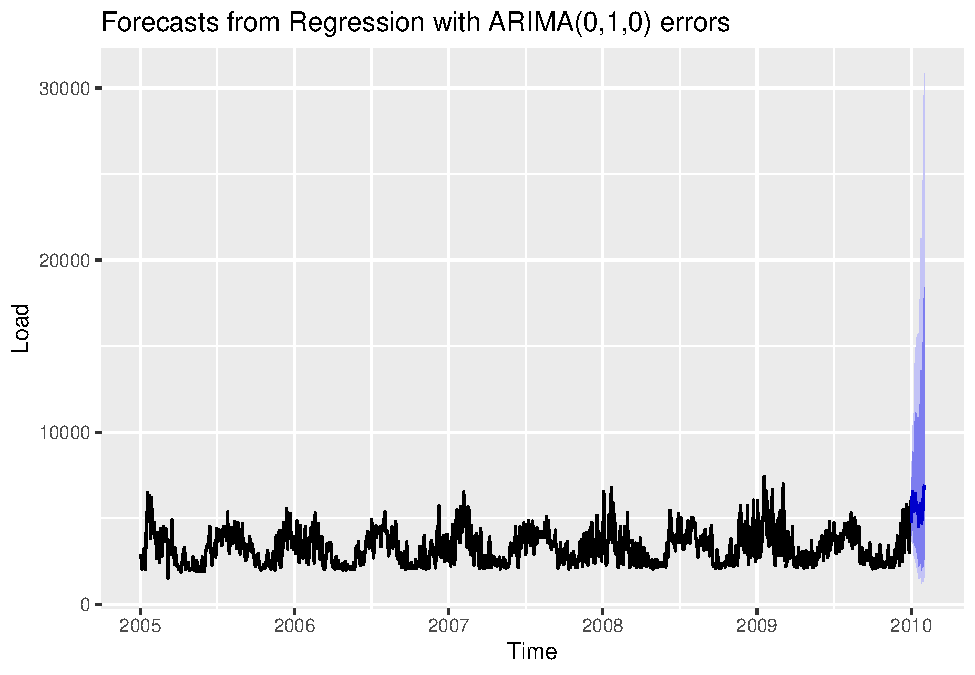
\includegraphics{ForecastCompetition_vFinal_files/figure-latex/unnamed-chunk-4-3.pdf}

\begin{Shaded}
\begin{Highlighting}[]
\CommentTok{\#Plot model + observed data}
\FunctionTok{autoplot}\NormalTok{(ts\_load\_compare) }\SpecialCharTok{+}
  \FunctionTok{autolayer}\NormalTok{(ARIMA\_Four\_for2, }\AttributeTok{series=}\StringTok{"ARIMA\_FOURIER\_Exogenous"}\NormalTok{,}\AttributeTok{PI=}\ConstantTok{FALSE}\NormalTok{) }\SpecialCharTok{+}
  \FunctionTok{ylab}\NormalTok{(}\StringTok{"Load"}\NormalTok{)}
\end{Highlighting}
\end{Shaded}

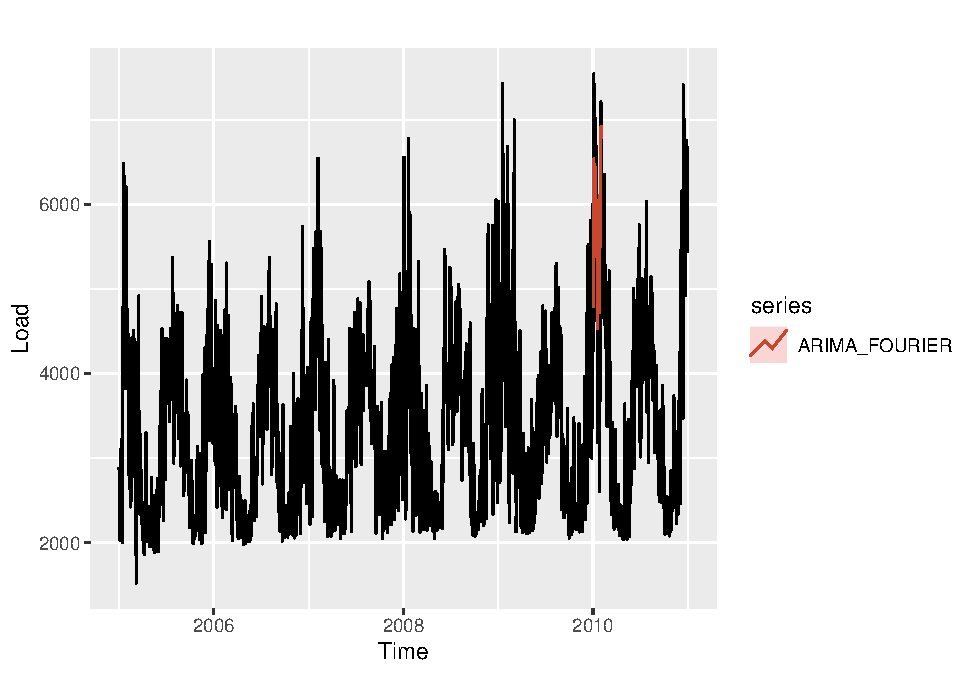
\includegraphics{ForecastCompetition_vFinal_files/figure-latex/unnamed-chunk-4-4.pdf}
\#\#ETS Model In this section, we fit and forecast the load data using
the STL+ETS model, plotted the forecast results, and compared it with
the observed data

\begin{Shaded}
\begin{Highlighting}[]
\CommentTok{\#Fit and forecast STL + ETS model to data}
\NormalTok{ETS\_fit }\OtherTok{\textless{}{-}}  \FunctionTok{stlf}\NormalTok{(ts\_load\_09,}\AttributeTok{h=}\DecValTok{31}\NormalTok{)}
\CommentTok{\#Plot foresting results}
\FunctionTok{autoplot}\NormalTok{(ETS\_fit) }\SpecialCharTok{+} \FunctionTok{ylab}\NormalTok{(}\StringTok{"Load"}\NormalTok{)}
\end{Highlighting}
\end{Shaded}

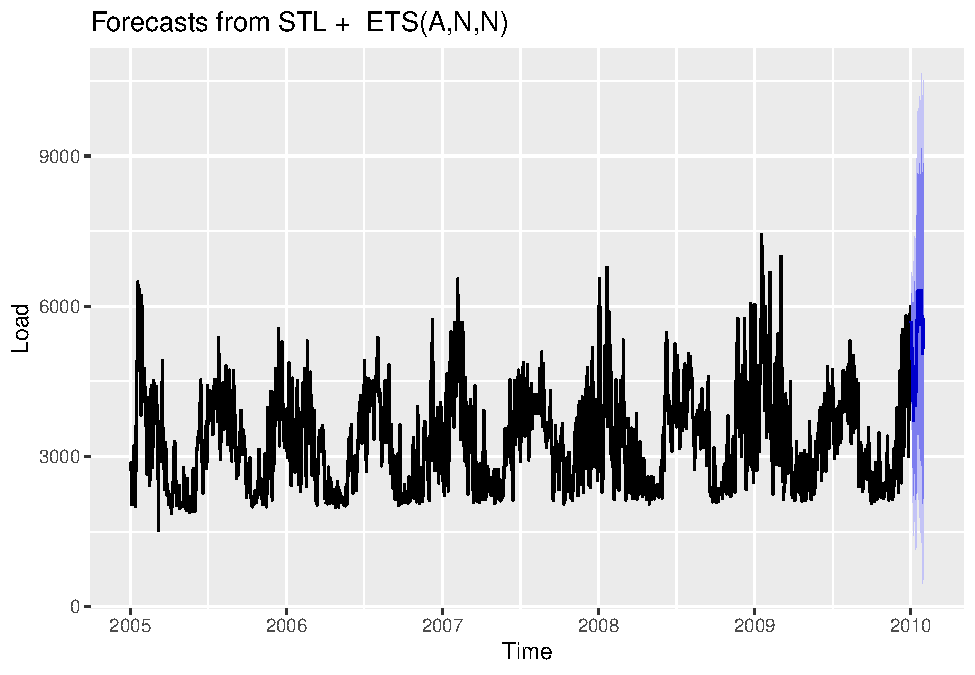
\includegraphics{ForecastCompetition_vFinal_files/figure-latex/unnamed-chunk-5-1.pdf}

\begin{Shaded}
\begin{Highlighting}[]
\CommentTok{\#Plot model + observed data}
\FunctionTok{autoplot}\NormalTok{(ts\_load\_compare) }\SpecialCharTok{+}
  \FunctionTok{autolayer}\NormalTok{(ETS\_fit, }\AttributeTok{series=}\StringTok{"STL + ETS"}\NormalTok{,}\AttributeTok{PI=}\ConstantTok{FALSE}\NormalTok{) }\SpecialCharTok{+}
  \FunctionTok{ylab}\NormalTok{(}\StringTok{"Load"}\NormalTok{)}
\end{Highlighting}
\end{Shaded}

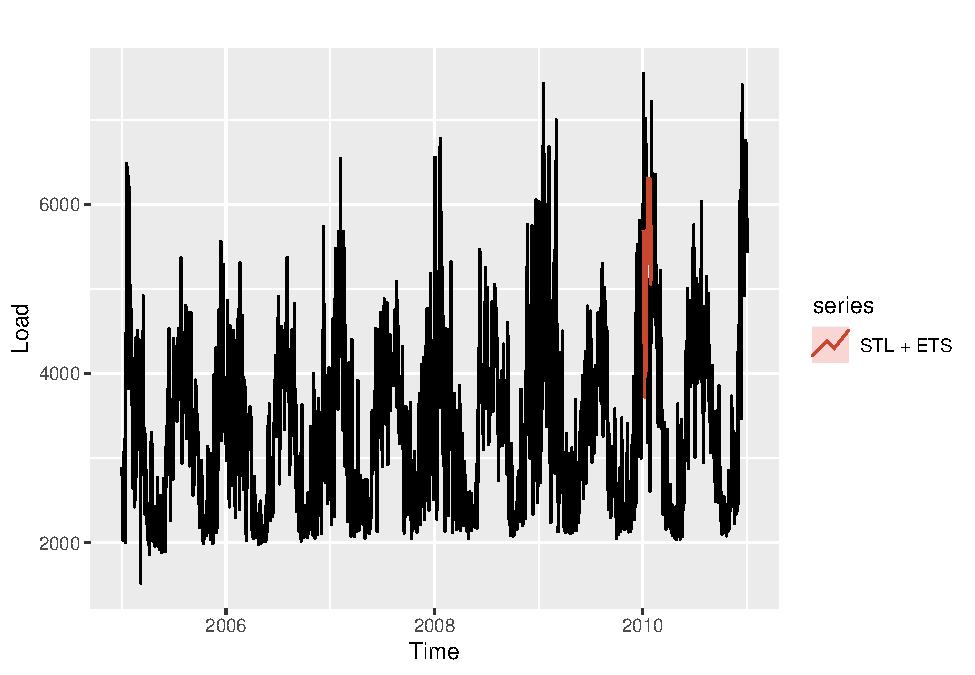
\includegraphics{ForecastCompetition_vFinal_files/figure-latex/unnamed-chunk-5-2.pdf}

\#\#TBATS Model In this section, we fit and forecast the load data using
the TBATS model, plotted the forecast results, and compared it with the
observed data

\begin{Shaded}
\begin{Highlighting}[]
\CommentTok{\# TBATS can take time to fit}
\NormalTok{TBATS\_fit }\OtherTok{\textless{}{-}} \FunctionTok{tbats}\NormalTok{(ts\_load\_09)}
\end{Highlighting}
\end{Shaded}

\begin{verbatim}
## Warning in tbats(ts_load_09): Missing values encountered. Using longest
## contiguous portion of time series
\end{verbatim}

\begin{Shaded}
\begin{Highlighting}[]
\NormalTok{TBATS\_for }\OtherTok{\textless{}{-}}\NormalTok{ forecast}\SpecialCharTok{::}\FunctionTok{forecast}\NormalTok{(TBATS\_fit, }\AttributeTok{h=}\DecValTok{31}\NormalTok{)}
\CommentTok{\#Plot foresting results}
\FunctionTok{autoplot}\NormalTok{(TBATS\_for) }\SpecialCharTok{+}
  \FunctionTok{ylab}\NormalTok{(}\StringTok{"Load"}\NormalTok{) }
\end{Highlighting}
\end{Shaded}

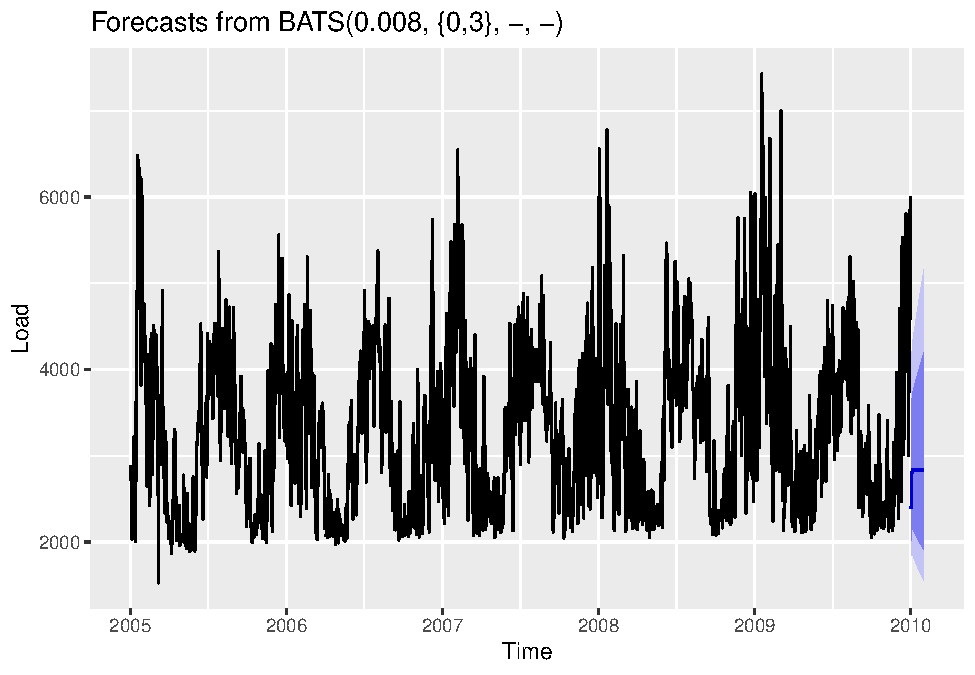
\includegraphics{ForecastCompetition_vFinal_files/figure-latex/unnamed-chunk-6-1.pdf}

\begin{Shaded}
\begin{Highlighting}[]
\CommentTok{\#Plot model + observed data}
\FunctionTok{autoplot}\NormalTok{(ts\_load\_compare) }\SpecialCharTok{+}
  \FunctionTok{autolayer}\NormalTok{(TBATS\_for, }\AttributeTok{series=}\StringTok{"TBATS"}\NormalTok{,}\AttributeTok{PI=}\ConstantTok{FALSE}\NormalTok{)}\SpecialCharTok{+}
  \FunctionTok{ylab}\NormalTok{(}\StringTok{"Load"}\NormalTok{) }
\end{Highlighting}
\end{Shaded}

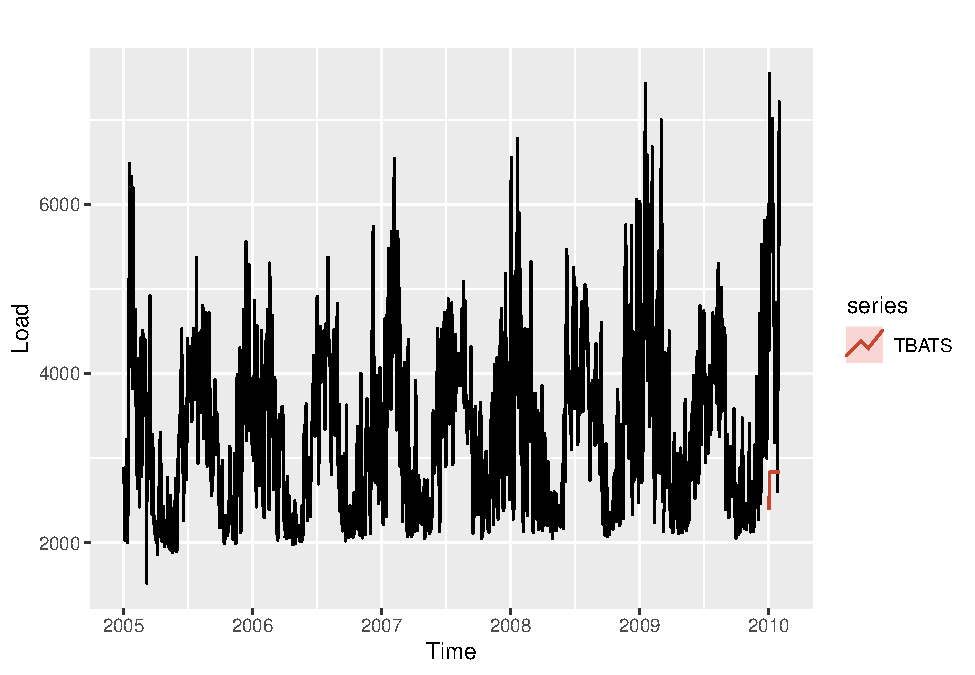
\includegraphics{ForecastCompetition_vFinal_files/figure-latex/unnamed-chunk-6-2.pdf}

\#\#Neural Network Similar analysis was conducted using the Neural
Network model. We used P=5 from the auto ARIMA model. We also ran a
model of a Neural Network with exogenous regressors and fourier terms.

\begin{Shaded}
\begin{Highlighting}[]
\CommentTok{\#NN\_fit }
\NormalTok{NN\_fit }\OtherTok{\textless{}{-}} \FunctionTok{nnetar}\NormalTok{(ts\_load\_09,}\AttributeTok{p=}\DecValTok{5}\NormalTok{,}\AttributeTok{P=}\DecValTok{0}\NormalTok{,}\AttributeTok{xreg=}\FunctionTok{fourier}\NormalTok{(ts\_load\_09, }\AttributeTok{K=}\FunctionTok{c}\NormalTok{(}\DecValTok{2}\NormalTok{,}\DecValTok{12}\NormalTok{)))}
\CommentTok{\#NN\_for }
\NormalTok{NN\_for }\OtherTok{\textless{}{-}}\NormalTok{ forecast}\SpecialCharTok{::}\FunctionTok{forecast}\NormalTok{(NN\_fit, }\AttributeTok{h=}\DecValTok{31}\NormalTok{,}\AttributeTok{xreg=}\FunctionTok{fourier}\NormalTok{(ts\_load\_09, }\AttributeTok{K=}\FunctionTok{c}\NormalTok{(}\DecValTok{2}\NormalTok{,}\DecValTok{12}\NormalTok{),}\AttributeTok{h=}\DecValTok{31}\NormalTok{))}
\CommentTok{\#Plot foresting results}
\FunctionTok{autoplot}\NormalTok{(NN\_for) }\SpecialCharTok{+}
  \FunctionTok{ylab}\NormalTok{(}\StringTok{"load"}\NormalTok{) }
\end{Highlighting}
\end{Shaded}

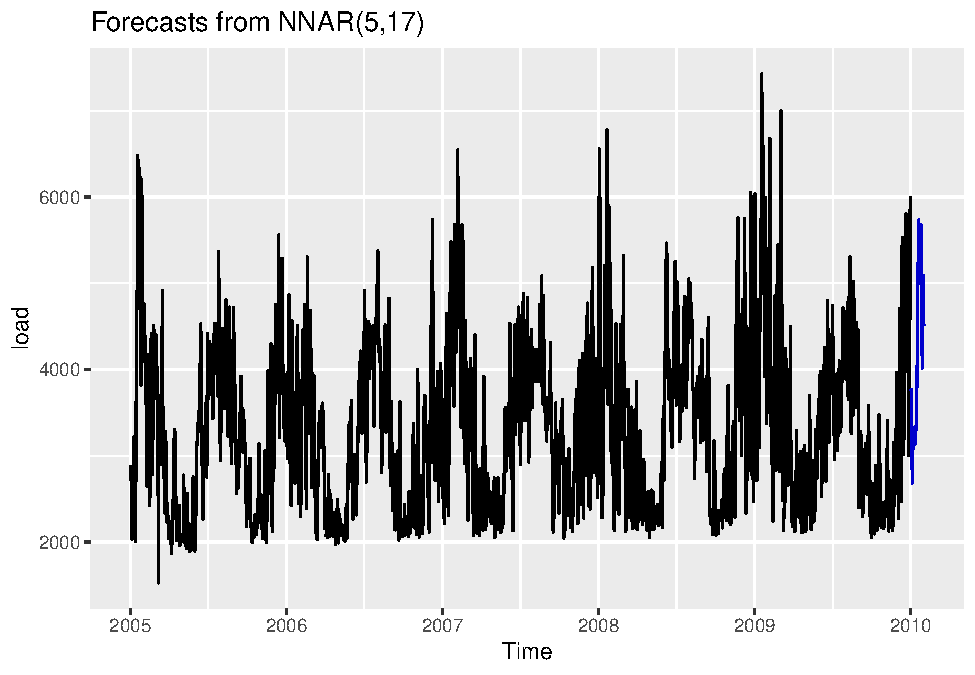
\includegraphics{ForecastCompetition_vFinal_files/figure-latex/unnamed-chunk-7-1.pdf}

\begin{Shaded}
\begin{Highlighting}[]
\CommentTok{\#Plot model + observed data}
\FunctionTok{autoplot}\NormalTok{(ts\_load\_compare) }\SpecialCharTok{+}
  \FunctionTok{autolayer}\NormalTok{(NN\_for, }\AttributeTok{series=}\StringTok{"Neural Network"}\NormalTok{,}\AttributeTok{PI=}\ConstantTok{FALSE}\NormalTok{)}\SpecialCharTok{+}
  \FunctionTok{ylab}\NormalTok{(}\StringTok{"load"}\NormalTok{) }
\end{Highlighting}
\end{Shaded}

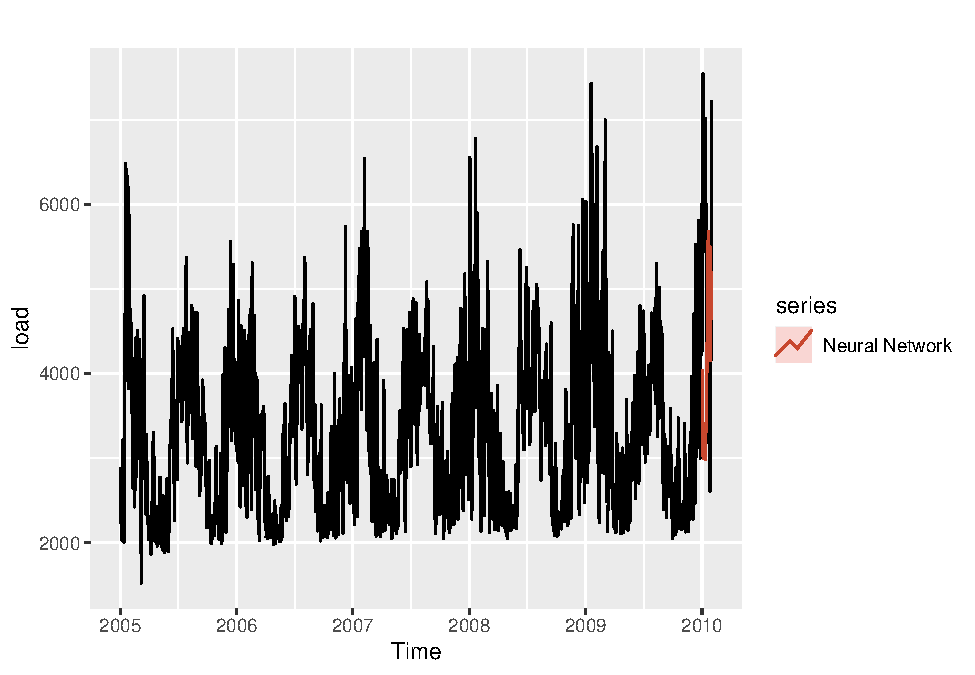
\includegraphics{ForecastCompetition_vFinal_files/figure-latex/unnamed-chunk-7-2.pdf}

\begin{Shaded}
\begin{Highlighting}[]
\DocumentationTok{\#\#with exogenous regressors and fourier}
\CommentTok{\#NN\_fit}
\NormalTok{NN\_fit2 }\OtherTok{\textless{}{-}} \FunctionTok{nnetar}\NormalTok{(ts\_load\_09,}\AttributeTok{p=}\DecValTok{5}\NormalTok{,}\AttributeTok{P=}\DecValTok{0}\NormalTok{,}\AttributeTok{xreg=}\NormalTok{xregs\_fourier)}
\CommentTok{\#NN\_for }
\NormalTok{NN\_for2 }\OtherTok{\textless{}{-}}\NormalTok{ forecast}\SpecialCharTok{::}\FunctionTok{forecast}\NormalTok{(NN\_fit2, }\AttributeTok{h=}\DecValTok{31}\NormalTok{,}\AttributeTok{xreg=}\NormalTok{xregs\_fourier\_for)}
\CommentTok{\#Plot foresting results}
\FunctionTok{autoplot}\NormalTok{(NN\_for2) }\SpecialCharTok{+}
  \FunctionTok{ylab}\NormalTok{(}\StringTok{"load"}\NormalTok{) }
\end{Highlighting}
\end{Shaded}

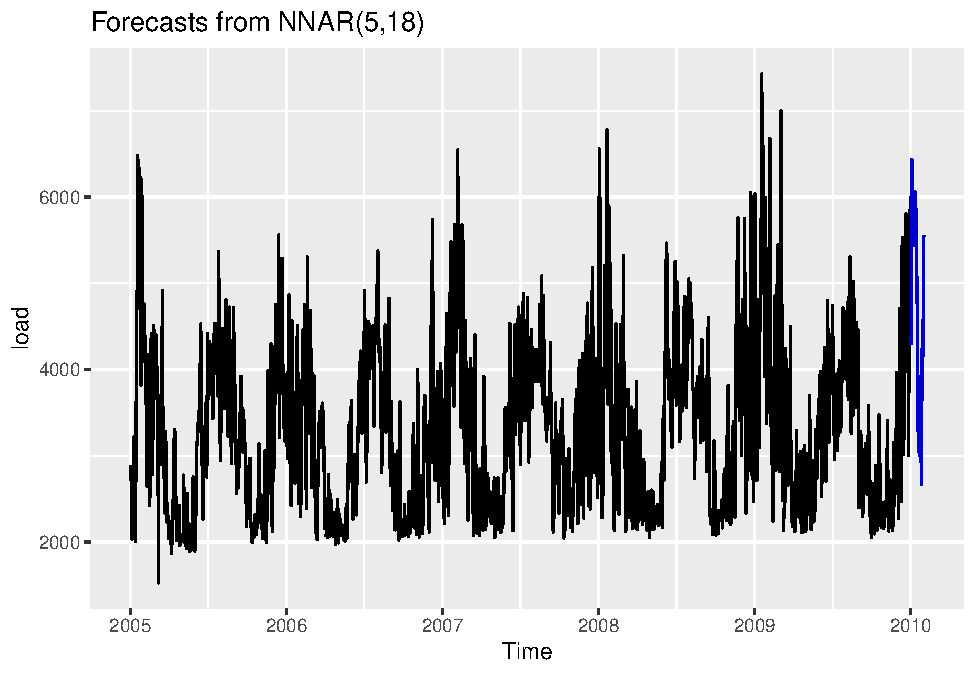
\includegraphics{ForecastCompetition_vFinal_files/figure-latex/unnamed-chunk-8-1.pdf}

\begin{Shaded}
\begin{Highlighting}[]
\CommentTok{\#Plot model + observed data}
\FunctionTok{autoplot}\NormalTok{(ts\_load\_compare) }\SpecialCharTok{+}
  \FunctionTok{autolayer}\NormalTok{(NN\_for2, }\AttributeTok{series=}\StringTok{"Neural Network with exogenous regressors"}\NormalTok{,}\AttributeTok{PI=}\ConstantTok{FALSE}\NormalTok{)}\SpecialCharTok{+}
  \FunctionTok{ylab}\NormalTok{(}\StringTok{"load"}\NormalTok{) }
\end{Highlighting}
\end{Shaded}

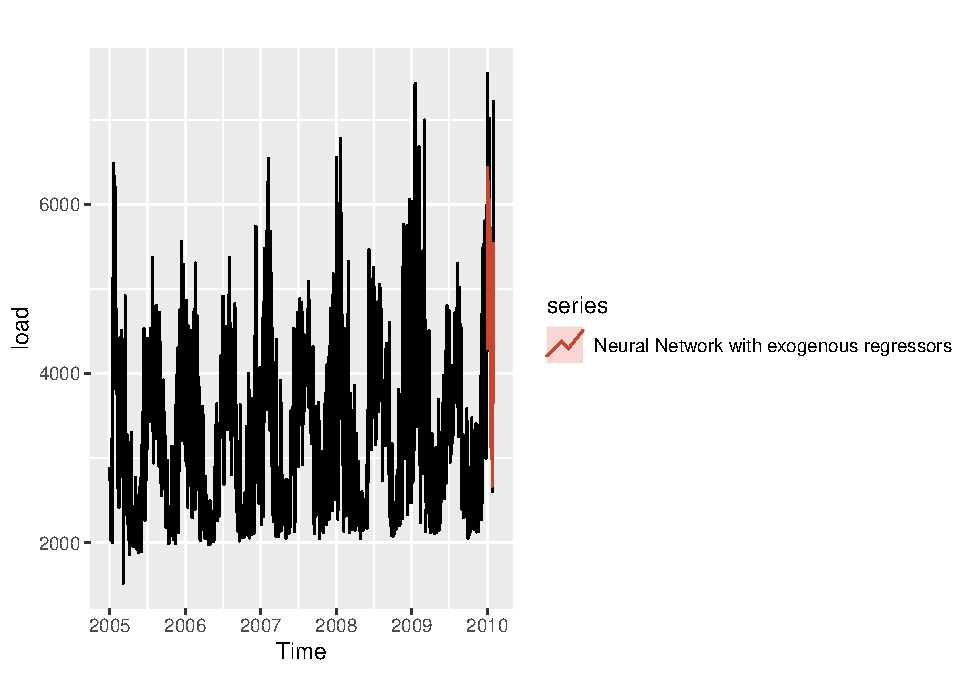
\includegraphics{ForecastCompetition_vFinal_files/figure-latex/unnamed-chunk-8-2.pdf}

\#\#Check Accuracy In this section, we checked the accuracy scores for
our models to compare the performance of our models. We ran 6 models in
total.

\begin{Shaded}
\begin{Highlighting}[]
\CommentTok{\#Model 1: STL + ETS}
\NormalTok{ETS\_scores }\OtherTok{\textless{}{-}} \FunctionTok{accuracy}\NormalTok{(ETS\_fit}\SpecialCharTok{$}\NormalTok{mean,ts\_load\_test)  }
\CommentTok{\#Model 2: ARIMA + Fourier }
\NormalTok{ARIMA\_scores }\OtherTok{\textless{}{-}} \FunctionTok{accuracy}\NormalTok{(ARIMA\_Four\_for}\SpecialCharTok{$}\NormalTok{mean,ts\_load\_test)}
\NormalTok{ARIMA\_scores2}\OtherTok{\textless{}{-}} \FunctionTok{accuracy}\NormalTok{(ARIMA\_Four\_for2}\SpecialCharTok{$}\NormalTok{mean,ts\_load\_test)}
\CommentTok{\# Model 3:  TBATS }
\NormalTok{TBATS\_scores }\OtherTok{\textless{}{-}} \FunctionTok{accuracy}\NormalTok{(TBATS\_for}\SpecialCharTok{$}\NormalTok{mean,ts\_load\_test)}
\CommentTok{\# Model 3:  Neural Network }
\NormalTok{NN\_scores }\OtherTok{\textless{}{-}} \FunctionTok{accuracy}\NormalTok{(NN\_for}\SpecialCharTok{$}\NormalTok{mean,ts\_load\_test)}
\NormalTok{NN\_scores2 }\OtherTok{\textless{}{-}} \FunctionTok{accuracy}\NormalTok{(NN\_for2}\SpecialCharTok{$}\NormalTok{mean,ts\_load\_test)}
\end{Highlighting}
\end{Shaded}

\hypertarget{check-residuals}{%
\subsection{Check Residuals}\label{check-residuals}}

We then plotted the residuals of our models to check for any sort of
bias. A model that accurately captures trend and seasonality should look
like uniform white noise. We see evidence of seasonality in STL+ETS,
ARIMA+Fourier, and Neural Networks as error bars in these residual plots
increase during winter months and decrease during summer months. The
addition of Xregs in the latter two models seems to eliminate the
seasonality and leaves residuals that are closer to true white noise.

\begin{Shaded}
\begin{Highlighting}[]
\FunctionTok{ts.plot}\NormalTok{(ETS\_fit}\SpecialCharTok{$}\NormalTok{residuals, }\AttributeTok{main=}\StringTok{"STL+ETS"}\NormalTok{)}
\end{Highlighting}
\end{Shaded}

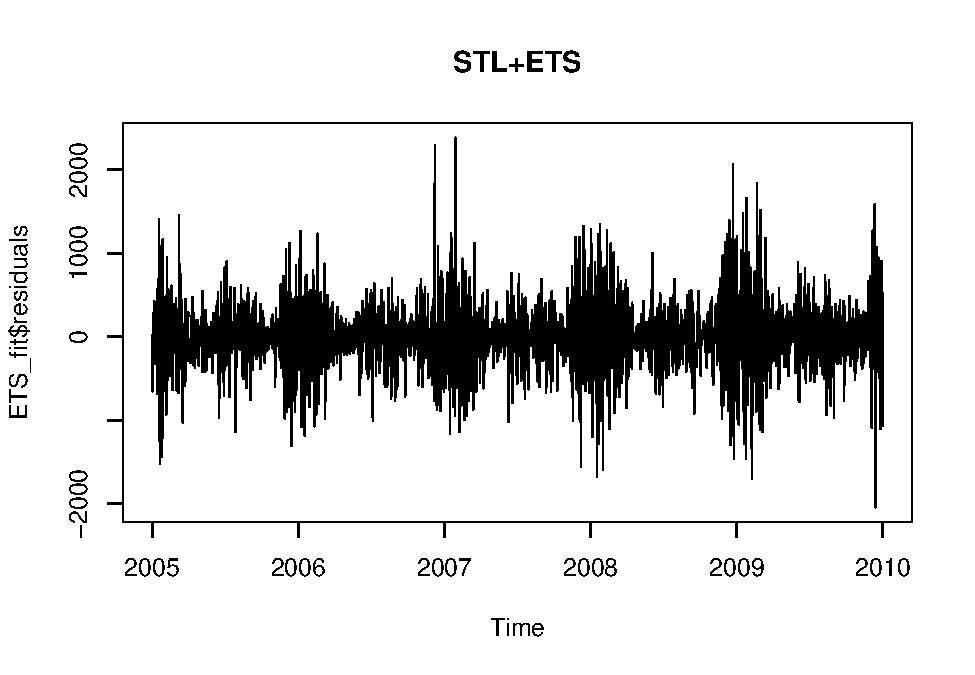
\includegraphics{ForecastCompetition_vFinal_files/figure-latex/check_residuals-1.pdf}

\begin{Shaded}
\begin{Highlighting}[]
\FunctionTok{ts.plot}\NormalTok{(ARIMA\_Four\_fit}\SpecialCharTok{$}\NormalTok{residuals, }\AttributeTok{main=}\StringTok{"ARIMA + Fourier"}\NormalTok{)}
\end{Highlighting}
\end{Shaded}

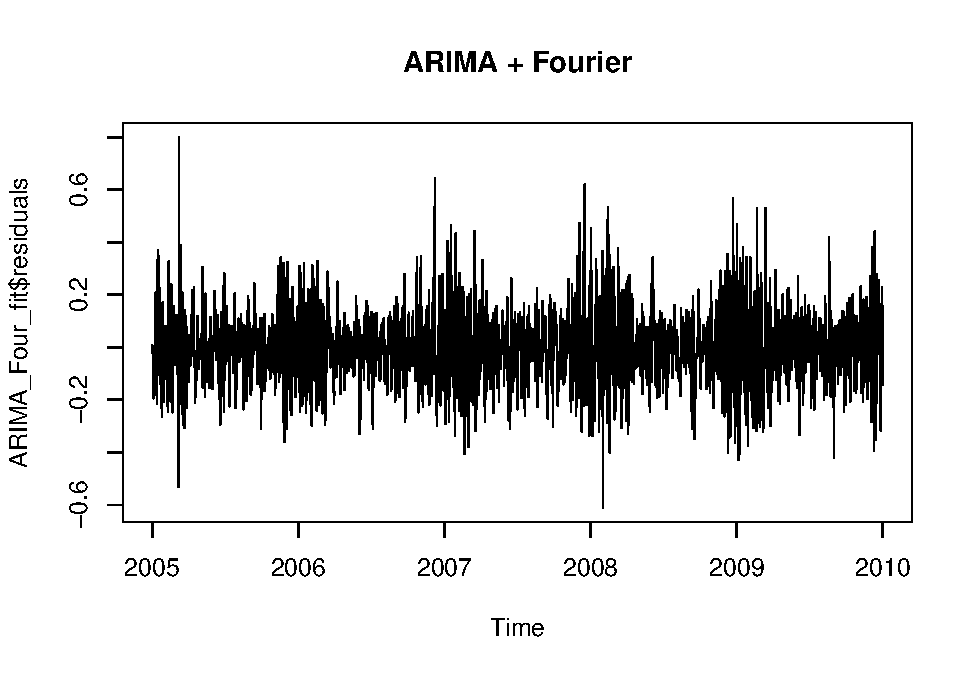
\includegraphics{ForecastCompetition_vFinal_files/figure-latex/check_residuals-2.pdf}

\begin{Shaded}
\begin{Highlighting}[]
\FunctionTok{ts.plot}\NormalTok{(ARIMA\_Four\_fit2}\SpecialCharTok{$}\NormalTok{residuals, }\AttributeTok{main=}\StringTok{"ARIMA+Fourier + Xregs"}\NormalTok{)}
\end{Highlighting}
\end{Shaded}

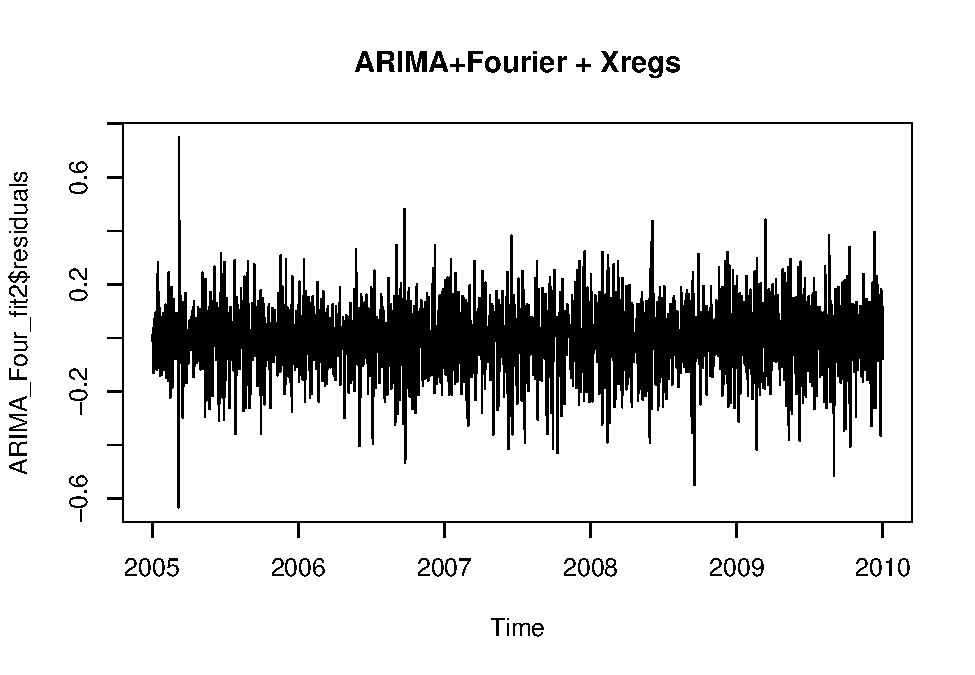
\includegraphics{ForecastCompetition_vFinal_files/figure-latex/check_residuals-3.pdf}

\begin{Shaded}
\begin{Highlighting}[]
\FunctionTok{ts.plot}\NormalTok{(TBATS\_for}\SpecialCharTok{$}\NormalTok{residuals, }\AttributeTok{main=}\StringTok{"TBATS"}\NormalTok{)}
\end{Highlighting}
\end{Shaded}

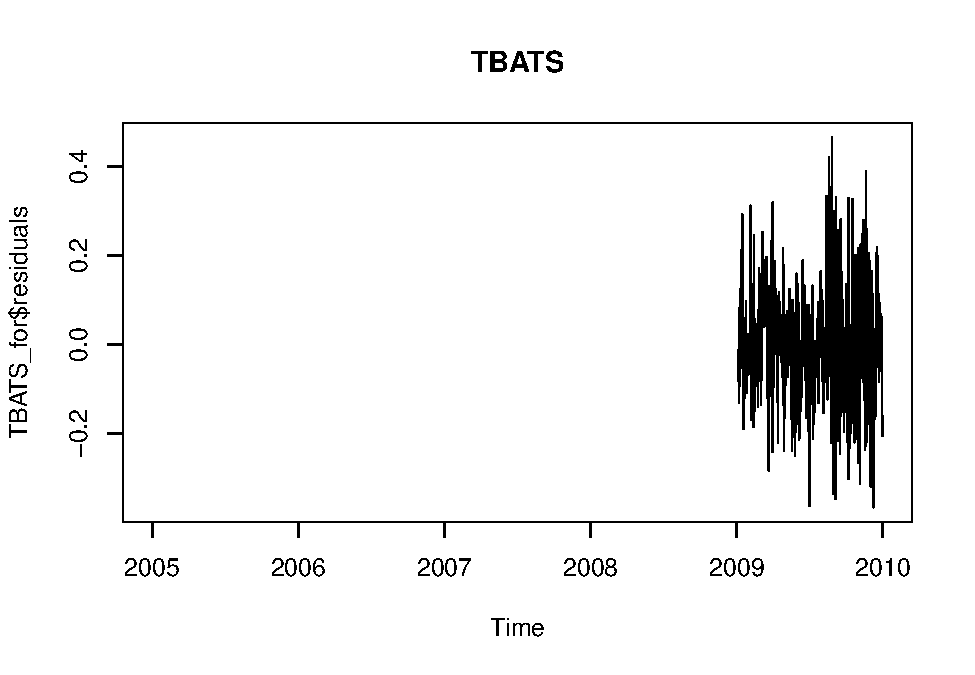
\includegraphics{ForecastCompetition_vFinal_files/figure-latex/check_residuals-4.pdf}

\begin{Shaded}
\begin{Highlighting}[]
\FunctionTok{ts.plot}\NormalTok{(NN\_fit}\SpecialCharTok{$}\NormalTok{residuals, }\AttributeTok{main=}\StringTok{"Neural Networks"}\NormalTok{)}
\end{Highlighting}
\end{Shaded}

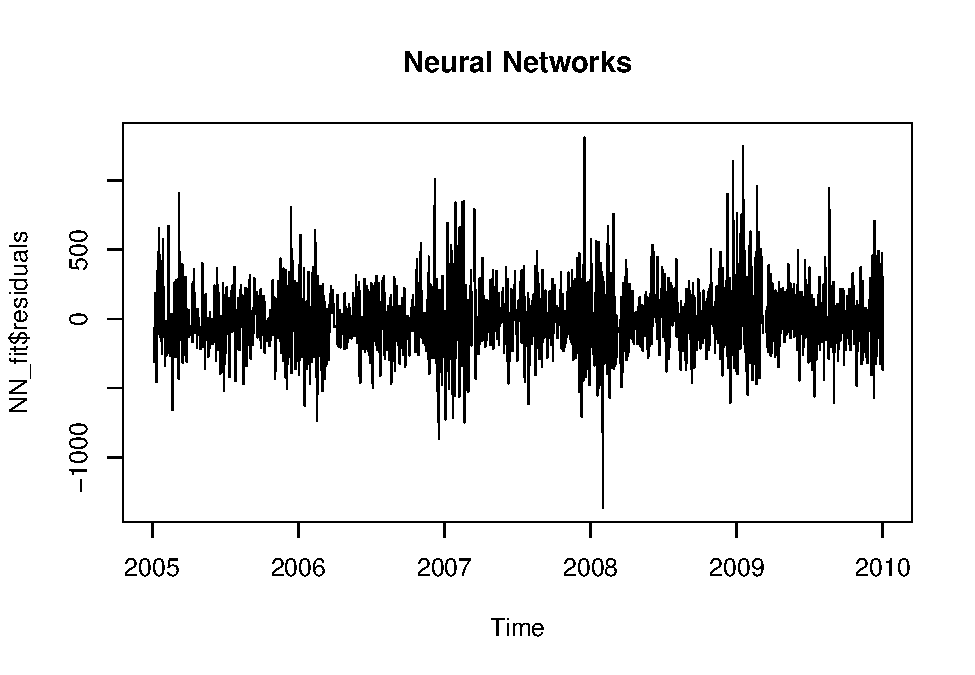
\includegraphics{ForecastCompetition_vFinal_files/figure-latex/check_residuals-5.pdf}

\begin{Shaded}
\begin{Highlighting}[]
\FunctionTok{ts.plot}\NormalTok{(NN\_fit2}\SpecialCharTok{$}\NormalTok{residuals, }\AttributeTok{main=}\StringTok{"Neural Networks + Xregs"}\NormalTok{)}
\end{Highlighting}
\end{Shaded}

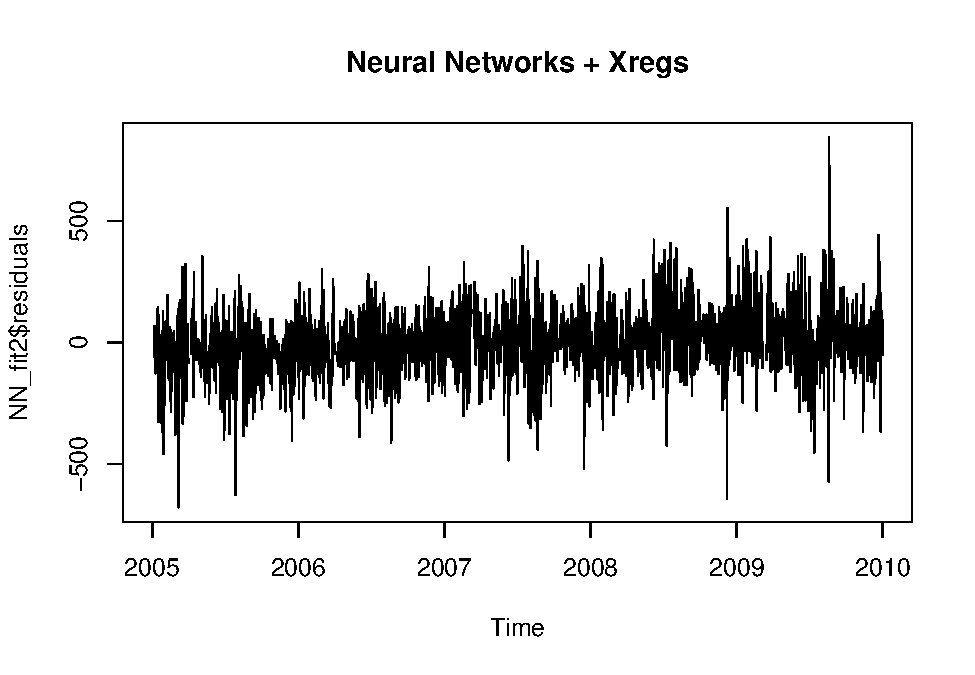
\includegraphics{ForecastCompetition_vFinal_files/figure-latex/check_residuals-6.pdf}

\#\#Comparing Performance Metrics

We compared performance metrics by creating a dataframe to hold all
performance metrics by model type. We also returned the model type with
the best RMSE score which was the neural network with exogenous
regressors. This was unsurprising as we saw that it produced a white
noise residuals plot.

\begin{Shaded}
\begin{Highlighting}[]
\CommentTok{\#create a dataframe of accuracy scores}
\NormalTok{scores }\OtherTok{\textless{}{-}} \FunctionTok{as.data.frame}\NormalTok{(}
  \FunctionTok{rbind}\NormalTok{(ETS\_scores, ARIMA\_scores,ARIMA\_scores2, TBATS\_scores, NN\_scores, NN\_scores2)}
\NormalTok{  )}
\FunctionTok{row.names}\NormalTok{(scores) }\OtherTok{\textless{}{-}} \FunctionTok{c}\NormalTok{(}\StringTok{"STL+ETS"}\NormalTok{, }\StringTok{"ARIMA+Fourier"}\NormalTok{, }\StringTok{"ARIMA+Fourier+XRegs"}\NormalTok{ ,}\StringTok{"TBATS"}\NormalTok{,}\StringTok{"NN"}\NormalTok{, }\StringTok{"NN+Xregs"}\NormalTok{)}

\CommentTok{\#choose model with lowest RMSE}
\NormalTok{best\_model\_index }\OtherTok{\textless{}{-}} \FunctionTok{which.min}\NormalTok{(scores[,}\StringTok{"RMSE"}\NormalTok{])}
\FunctionTok{cat}\NormalTok{(}\StringTok{"The best model by RMSE is:"}\NormalTok{, }\FunctionTok{row.names}\NormalTok{(scores[best\_model\_index,])) }
\end{Highlighting}
\end{Shaded}

\begin{verbatim}
## The best model by RMSE is: NN+Xregs
\end{verbatim}

\begin{Shaded}
\begin{Highlighting}[]
\FunctionTok{print}\NormalTok{(scores)}
\end{Highlighting}
\end{Shaded}

\begin{verbatim}
##                            ME      RMSE       MAE        MPE     MAPE      ACF1
## STL+ETS             -133.5084 1982.2491 1800.8504 -14.714124 40.30032 0.8423850
## ARIMA+Fourier       -288.9011 1981.2707 1782.4626 -17.596677 40.39527 0.8958187
## ARIMA+Fourier+XRegs -553.0001 1093.3194  905.4861 -17.077899 22.29190 0.8388483
## TBATS               2320.3354 2710.5455 2334.9495  40.469374 41.02927 0.7805849
## NN                   983.7291 2353.3242 2003.3297   7.943724 38.91544 0.8538864
## NN+Xregs             362.8663  645.7241  468.6570   5.919067  8.58528 0.4679727
##                     Theil's U
## STL+ETS             2.3892629
## ARIMA+Fourier       2.4948554
## ARIMA+Fourier+XRegs 1.5694497
## TBATS               2.4426533
## NN                  2.2753144
## NN+Xregs            0.6475376
\end{verbatim}

\#\#Finding Best Weather Stations

Upon closer investigation of the accuracy scores, we noticed that adding
the exogenous variables improved the accuracy scores of both our ARIMA
and Neural Networks models. Our approach to utilizing exogenous
variables by taking averages across all weather stations was fairly
rudimentary. Our next step was to try to improve upon our models by
taking a more descriminant approach to including exogenous variables.

In this chunk, we re-clean humidity and temperature data by creating
data frames holding averaging daily values for each weather station
rather than averaging the averages and getting only one variable for
humidity and one for temperature. Then we convert the dataframes to msts
and cbind with our load data to create a larger time series.

Then we find the correlation between each variable (load and humidity
and temperature for each of our weather stations) and print the names of
the weather stations that have the strongest correlations with load.
These are the weather stations that we will use to improve upon our
previous models.

The top 5 most correlated weather stations were all collecting
temperature, not humidity. This is unsurprising as temperature, not
humidity, is a more logical driver of electrical load than humidity
because people's behavior responds more to temperature.

\begin{Shaded}
\begin{Highlighting}[]
\CommentTok{\#Create new humidity dataframe with daily averages for every weather station}
\NormalTok{humidity\_3}\OtherTok{\textless{}{-}}\NormalTok{ humidity }\SpecialCharTok{\%\textgreater{}\%} 
  \FunctionTok{mutate}\NormalTok{( }\AttributeTok{Date =} \FunctionTok{ymd}\NormalTok{(date)) }\SpecialCharTok{\%\textgreater{}\%} 
  \FunctionTok{mutate}\NormalTok{( }\AttributeTok{Year =} \FunctionTok{year}\NormalTok{(date), }
          \AttributeTok{Month =} \FunctionTok{month}\NormalTok{(date), }
          \AttributeTok{Day =} \FunctionTok{day}\NormalTok{(date)) }\SpecialCharTok{\%\textgreater{}\%} 
  \FunctionTok{select}\NormalTok{( Date, Year, Month, Day, }\DecValTok{3}\SpecialCharTok{:}\DecValTok{33}\NormalTok{)}
\NormalTok{humidity\_daily\_2 }\OtherTok{\textless{}{-}}\NormalTok{ humidity\_3 }\SpecialCharTok{\%\textgreater{}\%} 
  \FunctionTok{group\_by}\NormalTok{(Date,Year,Month,Day) }\SpecialCharTok{\%\textgreater{}\%}
  \FunctionTok{summarise\_all}\NormalTok{(mean)}
\NormalTok{humidity\_daily\_2}\OtherTok{\textless{}{-}}\NormalTok{ humidity\_daily\_2[,(}\DecValTok{5}\SpecialCharTok{:}\DecValTok{33}\NormalTok{)]}

\CommentTok{\#Create new temp dataframe with daily averages for every weather station}
\NormalTok{temp\_3}\OtherTok{\textless{}{-}}\NormalTok{ temp }\SpecialCharTok{\%\textgreater{}\%} 
  \FunctionTok{mutate}\NormalTok{( }\AttributeTok{Date =} \FunctionTok{ymd}\NormalTok{(date)) }\SpecialCharTok{\%\textgreater{}\%} 
  \FunctionTok{mutate}\NormalTok{( }\AttributeTok{Year =} \FunctionTok{year}\NormalTok{(date), }
          \AttributeTok{Month =} \FunctionTok{month}\NormalTok{(date), }
          \AttributeTok{Day =} \FunctionTok{day}\NormalTok{(date)) }\SpecialCharTok{\%\textgreater{}\%} 
  \FunctionTok{select}\NormalTok{( Date, Year, Month, Day, }\DecValTok{3}\SpecialCharTok{:}\DecValTok{33}\NormalTok{)}
\NormalTok{temp\_daily\_2 }\OtherTok{\textless{}{-}}\NormalTok{ temp\_3 }\SpecialCharTok{\%\textgreater{}\%} 
  \FunctionTok{group\_by}\NormalTok{(Date,Year,Month,Day) }\SpecialCharTok{\%\textgreater{}\%}
  \FunctionTok{summarise\_all}\NormalTok{(mean)}
\NormalTok{temp\_daily\_2}\OtherTok{\textless{}{-}}\NormalTok{ temp\_daily\_2[,(}\DecValTok{5}\SpecialCharTok{:}\DecValTok{33}\NormalTok{)]}

\CommentTok{\#Make new xreg dataframes into msts and add to load msts}
\NormalTok{ts\_full\_humidity }\OtherTok{\textless{}{-}} \FunctionTok{msts}\NormalTok{(humidity\_daily\_2, }
                           \AttributeTok{seasonal.periods =}\FunctionTok{c}\NormalTok{(}\DecValTok{7}\NormalTok{,}\FloatTok{365.25}\NormalTok{),}
                           \AttributeTok{start=}\FunctionTok{c}\NormalTok{(}\DecValTok{2005}\NormalTok{,}\DecValTok{1}\NormalTok{,}\DecValTok{1}\NormalTok{))}
\NormalTok{ts\_full\_temp }\OtherTok{\textless{}{-}} \FunctionTok{msts}\NormalTok{(temp\_daily\_2, }
                           \AttributeTok{seasonal.periods =}\FunctionTok{c}\NormalTok{(}\DecValTok{7}\NormalTok{,}\FloatTok{365.25}\NormalTok{),}
                           \AttributeTok{start=}\FunctionTok{c}\NormalTok{(}\DecValTok{2005}\NormalTok{,}\DecValTok{1}\NormalTok{,}\DecValTok{1}\NormalTok{))}
\NormalTok{full\_data }\OtherTok{\textless{}{-}} \FunctionTok{cbind}\NormalTok{(ts\_load,ts\_full\_humidity,ts\_full\_temp)}

\CommentTok{\# Calculate the correlation between load and each weather station}
\NormalTok{corrmat }\OtherTok{\textless{}{-}} \FunctionTok{cor}\NormalTok{(full\_data[,}\DecValTok{1}\NormalTok{],full\_data[,}\SpecialCharTok{{-}}\DecValTok{1}\NormalTok{], }\AttributeTok{use =} \StringTok{"complete.obs"}\NormalTok{)}
\NormalTok{corrmat\_abs }\OtherTok{\textless{}{-}} \FunctionTok{abs}\NormalTok{(corrmat)}
\NormalTok{corrmat\_sorted }\OtherTok{\textless{}{-}}\NormalTok{ corrmat\_abs[,}\FunctionTok{order}\NormalTok{(corrmat\_abs[}\DecValTok{1}\NormalTok{,])]}

\CommentTok{\#Sort matrix and print the weather stations with highest absolute value correlation coefficients}
\NormalTok{top\_5\_corr }\OtherTok{\textless{}{-}} \FunctionTok{row.names}\NormalTok{(}\FunctionTok{as.data.frame}\NormalTok{(}\FunctionTok{tail}\NormalTok{(corrmat\_sorted,}\AttributeTok{n=}\DecValTok{5}\NormalTok{)))}
\FunctionTok{print}\NormalTok{(top\_5\_corr)}
\end{Highlighting}
\end{Shaded}

\begin{verbatim}
## [1] "ts_full_temp.t_ws25" "ts_full_temp.t_ws5"  "ts_full_temp.t_ws18"
## [4] "ts_full_temp.t_ws7"  "ts_full_temp.t_ws23"
\end{verbatim}

\hypertarget{create-new-fourierxregs-matrices}{%
\subsection{Create New Fourier+Xregs
Matrices}\label{create-new-fourierxregs-matrices}}

In this chunk, we create matrices that combine our fourier matrices and
the vectors of data from the 5 weather stations with highest absolute
value found in the previous chunk to be used to train new models and
forecast.

\begin{Shaded}
\begin{Highlighting}[]
\CommentTok{\#create matrix w fourier and 5 best correlations}
\NormalTok{xregs\_5\_best }\OtherTok{\textless{}{-}}\NormalTok{ temp\_daily\_2[,}\FunctionTok{c}\NormalTok{(}\DecValTok{25}\NormalTok{,}\DecValTok{5}\NormalTok{,}\DecValTok{18}\NormalTok{,}\DecValTok{7}\NormalTok{,}\DecValTok{23}\NormalTok{)]}
\NormalTok{xregs\_5\_best\_train }\OtherTok{\textless{}{-}}\NormalTok{ xregs\_5\_best[(}\DecValTok{1}\SpecialCharTok{:}\FunctionTok{nrow}\NormalTok{(fourier\_mat)),]}
\NormalTok{xregs\_best\_fourier}\OtherTok{\textless{}{-}}\FunctionTok{cbind}\NormalTok{(fourier\_mat,xregs\_5\_best\_train)}
\NormalTok{xregs\_best\_for}\OtherTok{\textless{}{-}}\NormalTok{xregs\_5\_best[(}\FunctionTok{nrow}\NormalTok{(xregs\_best\_fourier)}\SpecialCharTok{+}\DecValTok{1}\NormalTok{)}\SpecialCharTok{:}\NormalTok{(}\FunctionTok{nrow}\NormalTok{(xregs\_best\_fourier)}\SpecialCharTok{+}\DecValTok{31}\NormalTok{),]}
\NormalTok{xregs\_best\_fourier\_for}\OtherTok{\textless{}{-}}\FunctionTok{cbind}\NormalTok{(fourier\_mat\_for,xregs\_best\_for)}
\end{Highlighting}
\end{Shaded}

\#\#Rerunning Neural Networks with best weather stations

Our next is to utilize our fourier terms and our 5 best exogenous
regressors to rerun the neural network model and forecast. Our residuals
look similarly unbiased as before. Our RMSE has improved as we had
hoped.

\begin{Shaded}
\begin{Highlighting}[]
\DocumentationTok{\#\#Run neural network with top 5 weather stations and fourier}
\NormalTok{NN\_fit3 }\OtherTok{\textless{}{-}} \FunctionTok{nnetar}\NormalTok{(ts\_load\_09,}\AttributeTok{p=}\DecValTok{5}\NormalTok{,}\AttributeTok{P=}\DecValTok{0}\NormalTok{,}\AttributeTok{xreg=}\NormalTok{xregs\_best\_fourier)}
\NormalTok{NN\_for3 }\OtherTok{\textless{}{-}}\NormalTok{ forecast}\SpecialCharTok{::}\FunctionTok{forecast}\NormalTok{(NN\_fit3, }\AttributeTok{h=}\DecValTok{31}\NormalTok{,}\AttributeTok{xreg=}\NormalTok{xregs\_best\_fourier\_for)}

\CommentTok{\#Plot}
\FunctionTok{autoplot}\NormalTok{(NN\_for3, }\AttributeTok{main=}\StringTok{"Neural Network w Best Xregs"}\NormalTok{) }\SpecialCharTok{+} \FunctionTok{ylab}\NormalTok{(}\StringTok{"load"}\NormalTok{)}
\end{Highlighting}
\end{Shaded}

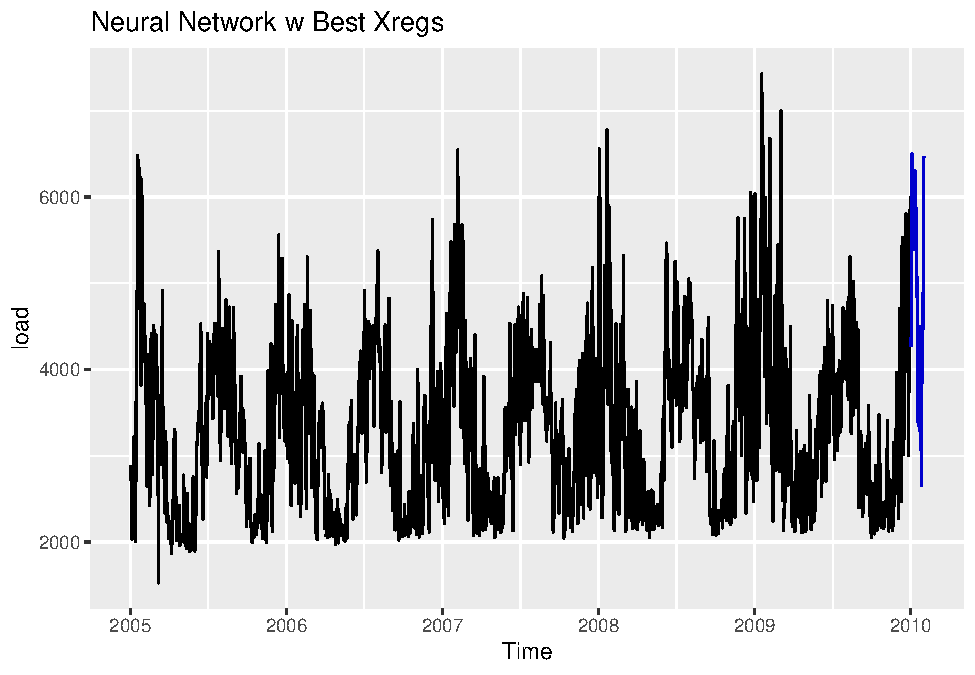
\includegraphics{ForecastCompetition_vFinal_files/figure-latex/NN_bestXregs-1.pdf}

\begin{Shaded}
\begin{Highlighting}[]
\CommentTok{\#Plot residuals}
\FunctionTok{ts.plot}\NormalTok{(NN\_fit3}\SpecialCharTok{$}\NormalTok{residuals, }\AttributeTok{main=}\StringTok{"Neural Networks + Best Xregs Residuals"}\NormalTok{)}
\end{Highlighting}
\end{Shaded}

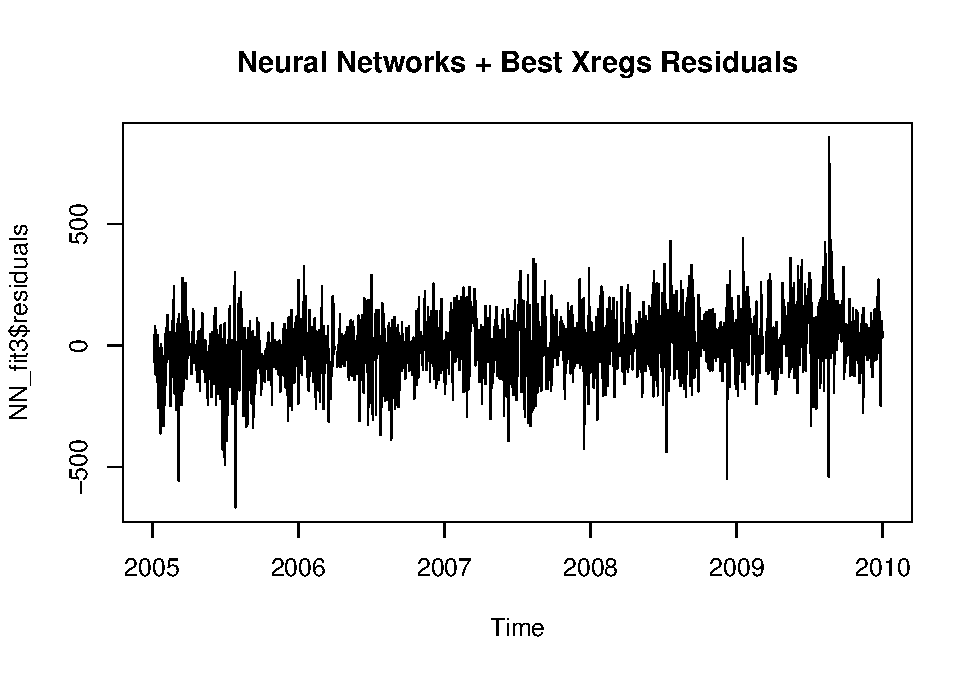
\includegraphics{ForecastCompetition_vFinal_files/figure-latex/NN_bestXregs-2.pdf}

\begin{Shaded}
\begin{Highlighting}[]
\CommentTok{\#Accuracy Test}
\NormalTok{NN\_scores3 }\OtherTok{\textless{}{-}} \FunctionTok{accuracy}\NormalTok{(NN\_for3}\SpecialCharTok{$}\NormalTok{mean,ts\_load\_test)}
\FunctionTok{print}\NormalTok{(NN\_scores3)}
\end{Highlighting}
\end{Shaded}

\begin{verbatim}
##                ME     RMSE      MAE      MPE     MAPE      ACF1 Theil's U
## Test set 209.9717 428.4372 291.2903 3.151418 5.079237 0.4099622 0.4217102
\end{verbatim}

\hypertarget{define-fourier-and-xregs-matrices-for-jan-11-train-and-forecast}{%
\subsection{Define Fourier and Xregs Matrices for Jan '11 Train and
Forecast}\label{define-fourier-and-xregs-matrices-for-jan-11-train-and-forecast}}

Then we generated training and forecasting matrices of our fourier terms
and exogenous regressors.

\begin{Shaded}
\begin{Highlighting}[]
\NormalTok{fourier\_mat\_10\_train }\OtherTok{\textless{}{-}} \FunctionTok{fourier}\NormalTok{(ts\_load,}\AttributeTok{K=}\FunctionTok{c}\NormalTok{(}\DecValTok{2}\NormalTok{,}\DecValTok{12}\NormalTok{),}\AttributeTok{h=}\FunctionTok{nrow}\NormalTok{(ts\_load))}
\NormalTok{fourier\_mat\_10\_for}\OtherTok{\textless{}{-}}\FunctionTok{fourier}\NormalTok{(ts\_load,}\AttributeTok{K=}\FunctionTok{c}\NormalTok{(}\DecValTok{2}\NormalTok{,}\DecValTok{12}\NormalTok{),}\AttributeTok{h=}\DecValTok{31}\NormalTok{)}
\NormalTok{xregs\_best\_four\_mat\_10 }\OtherTok{\textless{}{-}} \FunctionTok{cbind}\NormalTok{(fourier\_mat\_10\_train,xregs\_5\_best)}
\end{Highlighting}
\end{Shaded}

\hypertarget{forecast-xregs-for-use-in-load-forecast}{%
\subsection{Forecast Xregs for Use in Load
Forecast}\label{forecast-xregs-for-use-in-load-forecast}}

We then forecasted our exogenous variables so we could use them to
forecast the load for January 2011. We first utilized auto.arima models
to forecast each of our 5 most correlated temperature variables with
load and then our average temperature and humidity across alll weather
stations. The plots of these forecasts are shown below.

\begin{Shaded}
\begin{Highlighting}[]
\CommentTok{\# forecast xregs}
\NormalTok{ARIMA\_Four\_fit\_xreg1 }\OtherTok{\textless{}{-}} \FunctionTok{auto.arima}\NormalTok{(xregs\_5\_best}\SpecialCharTok{$}\NormalTok{t\_ws25, }\AttributeTok{seasonal=}\ConstantTok{FALSE}\NormalTok{, }\AttributeTok{lambda=}\DecValTok{0}\NormalTok{,}\AttributeTok{xreg=}\NormalTok{fourier\_mat\_10\_train)}
\NormalTok{ARIMA\_Four\_fit\_xreg2 }\OtherTok{\textless{}{-}} \FunctionTok{auto.arima}\NormalTok{(xregs\_5\_best}\SpecialCharTok{$}\NormalTok{t\_ws5, }\AttributeTok{seasonal=}\ConstantTok{FALSE}\NormalTok{, }\AttributeTok{lambda=}\DecValTok{0}\NormalTok{,}\AttributeTok{xreg=}\NormalTok{fourier\_mat\_10\_train)}
\NormalTok{ARIMA\_Four\_fit\_xreg3 }\OtherTok{\textless{}{-}} \FunctionTok{auto.arima}\NormalTok{(xregs\_5\_best}\SpecialCharTok{$}\NormalTok{t\_ws18, }\AttributeTok{seasonal=}\ConstantTok{FALSE}\NormalTok{, }\AttributeTok{lambda=}\DecValTok{0}\NormalTok{,}\AttributeTok{xreg=}\NormalTok{fourier\_mat\_10\_train)}
\NormalTok{ARIMA\_Four\_fit\_xreg4 }\OtherTok{\textless{}{-}} \FunctionTok{auto.arima}\NormalTok{(xregs\_5\_best}\SpecialCharTok{$}\NormalTok{t\_ws7, }\AttributeTok{seasonal=}\ConstantTok{FALSE}\NormalTok{, }\AttributeTok{lambda=}\DecValTok{0}\NormalTok{,}\AttributeTok{xreg=}\NormalTok{fourier\_mat\_10\_train)}
\NormalTok{ARIMA\_Four\_fit\_xreg5 }\OtherTok{\textless{}{-}} \FunctionTok{auto.arima}\NormalTok{(xregs\_5\_best}\SpecialCharTok{$}\NormalTok{t\_ws23, }\AttributeTok{seasonal=}\ConstantTok{FALSE}\NormalTok{, }\AttributeTok{lambda=}\DecValTok{0}\NormalTok{,}\AttributeTok{xreg=}\NormalTok{fourier\_mat\_10\_train)}
\NormalTok{ARIMA\_Four\_fit\_xreg\_Ave\_temp }\OtherTok{\textless{}{-}} \FunctionTok{auto.arima}\NormalTok{(xregs\_daily[,}\DecValTok{1}\NormalTok{], }\AttributeTok{seasonal=}\ConstantTok{FALSE}\NormalTok{, }\AttributeTok{lambda=}\DecValTok{0}\NormalTok{,}\AttributeTok{xreg=}\NormalTok{fourier\_mat\_10\_train)}
\NormalTok{ARIMA\_Four\_fit\_xreg\_Ave\_humidity }\OtherTok{\textless{}{-}} \FunctionTok{auto.arima}\NormalTok{(xregs\_daily[,}\DecValTok{2}\NormalTok{], }\AttributeTok{seasonal=}\ConstantTok{FALSE}\NormalTok{, }\AttributeTok{lambda=}\DecValTok{0}\NormalTok{,}\AttributeTok{xreg=}\NormalTok{fourier\_mat\_10\_train)}

\CommentTok{\#Forecast with ARIMA fit}
\CommentTok{\#also need to specify h for fourier terms}
\NormalTok{ARIMA\_Four\_for\_xreg1 }\OtherTok{\textless{}{-}}\NormalTok{ forecast}\SpecialCharTok{::}\FunctionTok{forecast}\NormalTok{(ARIMA\_Four\_fit\_xreg1, }\AttributeTok{xreg=}\NormalTok{fourier\_mat\_10\_for, }\AttributeTok{h=}\DecValTok{31}\NormalTok{) }
\NormalTok{ARIMA\_Four\_for\_xreg2 }\OtherTok{\textless{}{-}}\NormalTok{ forecast}\SpecialCharTok{::}\FunctionTok{forecast}\NormalTok{(ARIMA\_Four\_fit\_xreg2, }\AttributeTok{xreg=}\NormalTok{fourier\_mat\_10\_for, }\AttributeTok{h=}\DecValTok{31}\NormalTok{) }
\NormalTok{ARIMA\_Four\_for\_xreg3 }\OtherTok{\textless{}{-}}\NormalTok{ forecast}\SpecialCharTok{::}\FunctionTok{forecast}\NormalTok{(ARIMA\_Four\_fit\_xreg3, }\AttributeTok{xreg=}\NormalTok{fourier\_mat\_10\_for, }\AttributeTok{h=}\DecValTok{31}\NormalTok{) }
\NormalTok{ARIMA\_Four\_for\_xreg4 }\OtherTok{\textless{}{-}}\NormalTok{ forecast}\SpecialCharTok{::}\FunctionTok{forecast}\NormalTok{(ARIMA\_Four\_fit\_xreg4, }\AttributeTok{xreg=}\NormalTok{fourier\_mat\_10\_for, }\AttributeTok{h=}\DecValTok{31}\NormalTok{) }
\NormalTok{ARIMA\_Four\_for\_xreg5 }\OtherTok{\textless{}{-}}\NormalTok{ forecast}\SpecialCharTok{::}\FunctionTok{forecast}\NormalTok{(ARIMA\_Four\_fit\_xreg5, }\AttributeTok{xreg=}\NormalTok{fourier\_mat\_10\_for, }\AttributeTok{h=}\DecValTok{31}\NormalTok{) }
\NormalTok{ARIMA\_Four\_for\_xreg\_Ave\_temp }\OtherTok{\textless{}{-}}\NormalTok{ forecast}\SpecialCharTok{::}\FunctionTok{forecast}\NormalTok{(ARIMA\_Four\_fit\_xreg\_Ave\_temp, }\AttributeTok{xreg=}\NormalTok{fourier\_mat\_10\_for, }\AttributeTok{h=}\DecValTok{31}\NormalTok{) }
\NormalTok{ARIMA\_Four\_for\_xreg\_Ave\_humidity }\OtherTok{\textless{}{-}}\NormalTok{ forecast}\SpecialCharTok{::}\FunctionTok{forecast}\NormalTok{(ARIMA\_Four\_fit\_xreg\_Ave\_humidity, }\AttributeTok{xreg=}\NormalTok{fourier\_mat\_10\_for, }\AttributeTok{h=}\DecValTok{31}\NormalTok{) }

\FunctionTok{autoplot}\NormalTok{(ARIMA\_Four\_for\_xreg1) }\SpecialCharTok{+} \FunctionTok{ylab}\NormalTok{(}\StringTok{"Temp"}\NormalTok{)}
\end{Highlighting}
\end{Shaded}

\includegraphics{ForecastCompetition_vFinal_files/figure-latex/arima_xreg_forecast-1.pdf}

\begin{Shaded}
\begin{Highlighting}[]
\FunctionTok{autoplot}\NormalTok{(ARIMA\_Four\_for\_xreg2) }\SpecialCharTok{+} \FunctionTok{ylab}\NormalTok{(}\StringTok{"Temp"}\NormalTok{)}
\end{Highlighting}
\end{Shaded}

\includegraphics{ForecastCompetition_vFinal_files/figure-latex/arima_xreg_forecast-2.pdf}

\begin{Shaded}
\begin{Highlighting}[]
\FunctionTok{autoplot}\NormalTok{(ARIMA\_Four\_for\_xreg3) }\SpecialCharTok{+} \FunctionTok{ylab}\NormalTok{(}\StringTok{"Temp"}\NormalTok{)}
\end{Highlighting}
\end{Shaded}

\includegraphics{ForecastCompetition_vFinal_files/figure-latex/arima_xreg_forecast-3.pdf}

\begin{Shaded}
\begin{Highlighting}[]
\FunctionTok{autoplot}\NormalTok{(ARIMA\_Four\_for\_xreg4) }\SpecialCharTok{+} \FunctionTok{ylab}\NormalTok{(}\StringTok{"Temp"}\NormalTok{)}
\end{Highlighting}
\end{Shaded}

\includegraphics{ForecastCompetition_vFinal_files/figure-latex/arima_xreg_forecast-4.pdf}

\begin{Shaded}
\begin{Highlighting}[]
\FunctionTok{autoplot}\NormalTok{(ARIMA\_Four\_for\_xreg5) }\SpecialCharTok{+} \FunctionTok{ylab}\NormalTok{(}\StringTok{"Temp"}\NormalTok{)}
\end{Highlighting}
\end{Shaded}

\includegraphics{ForecastCompetition_vFinal_files/figure-latex/arima_xreg_forecast-5.pdf}

\begin{Shaded}
\begin{Highlighting}[]
\FunctionTok{autoplot}\NormalTok{(ARIMA\_Four\_for\_xreg\_Ave\_temp) }\SpecialCharTok{+} \FunctionTok{ylab}\NormalTok{(}\StringTok{"Temp"}\NormalTok{)}
\end{Highlighting}
\end{Shaded}

\includegraphics{ForecastCompetition_vFinal_files/figure-latex/arima_xreg_forecast-6.pdf}

\begin{Shaded}
\begin{Highlighting}[]
\FunctionTok{autoplot}\NormalTok{(ARIMA\_Four\_for\_xreg\_Ave\_humidity) }\SpecialCharTok{+} \FunctionTok{ylab}\NormalTok{(}\StringTok{"Humidity"}\NormalTok{)}
\end{Highlighting}
\end{Shaded}

\includegraphics{ForecastCompetition_vFinal_files/figure-latex/arima_xreg_forecast-7.pdf}

\hypertarget{nn-forecast-xregs-for-use-in-load-forecast}{%
\subsection{NN Forecast Xregs for Use in Load
Forecast}\label{nn-forecast-xregs-for-use-in-load-forecast}}

Then we used the p order generated from the auto.arimas to run neural
network forecasts of each of the exogenous regressors. Plots shown
below.

\begin{Shaded}
\begin{Highlighting}[]
\CommentTok{\#Running NN for xregs using the p produced from Auto.ARIMAs}
\NormalTok{NN\_fit\_xreg1 }\OtherTok{\textless{}{-}} \FunctionTok{nnetar}\NormalTok{(xregs\_5\_best}\SpecialCharTok{$}\NormalTok{t\_ws25,}\AttributeTok{p=}\DecValTok{1}\NormalTok{,}\AttributeTok{P=}\DecValTok{0}\NormalTok{,}\AttributeTok{xreg=}\NormalTok{fourier\_mat\_10\_train)}
\NormalTok{NN\_fit\_xreg2 }\OtherTok{\textless{}{-}} \FunctionTok{nnetar}\NormalTok{(xregs\_5\_best}\SpecialCharTok{$}\NormalTok{t\_ws5,}\AttributeTok{p=}\DecValTok{4}\NormalTok{,}\AttributeTok{P=}\DecValTok{0}\NormalTok{,}\AttributeTok{xreg=}\NormalTok{fourier\_mat\_10\_train)}
\NormalTok{NN\_fit\_xreg3 }\OtherTok{\textless{}{-}} \FunctionTok{nnetar}\NormalTok{(xregs\_5\_best}\SpecialCharTok{$}\NormalTok{t\_ws18,}\AttributeTok{p=}\DecValTok{1}\NormalTok{,}\AttributeTok{P=}\DecValTok{0}\NormalTok{,}\AttributeTok{xreg=}\NormalTok{fourier\_mat\_10\_train)}
\NormalTok{NN\_fit\_xreg4 }\OtherTok{\textless{}{-}} \FunctionTok{nnetar}\NormalTok{(xregs\_5\_best}\SpecialCharTok{$}\NormalTok{t\_ws7,}\AttributeTok{p=}\DecValTok{3}\NormalTok{,}\AttributeTok{P=}\DecValTok{0}\NormalTok{,}\AttributeTok{xreg=}\NormalTok{fourier\_mat\_10\_train)}
\NormalTok{NN\_fit\_xreg5 }\OtherTok{\textless{}{-}} \FunctionTok{nnetar}\NormalTok{(xregs\_5\_best}\SpecialCharTok{$}\NormalTok{t\_ws23,}\AttributeTok{p=}\DecValTok{1}\NormalTok{,}\AttributeTok{P=}\DecValTok{0}\NormalTok{,}\AttributeTok{xreg=}\NormalTok{fourier\_mat\_10\_train)}
\NormalTok{NN\_fit\_xreg\_ave\_temp }\OtherTok{\textless{}{-}} \FunctionTok{nnetar}\NormalTok{(xregs\_daily[,}\DecValTok{1}\NormalTok{],}\AttributeTok{p=}\DecValTok{5}\NormalTok{,}\AttributeTok{P=}\DecValTok{0}\NormalTok{,}\AttributeTok{xreg=}\NormalTok{fourier\_mat\_10\_train)}
\NormalTok{NN\_fit\_xreg\_ave\_humidity }\OtherTok{\textless{}{-}} \FunctionTok{nnetar}\NormalTok{(xregs\_daily[,}\DecValTok{2}\NormalTok{],}\AttributeTok{p=}\DecValTok{2}\NormalTok{,}\AttributeTok{P=}\DecValTok{0}\NormalTok{,}\AttributeTok{xreg=}\NormalTok{fourier\_mat\_10\_train)}

\CommentTok{\#Forecasts}
\NormalTok{NN\_for\_xreg1 }\OtherTok{\textless{}{-}}\NormalTok{ forecast}\SpecialCharTok{::}\FunctionTok{forecast}\NormalTok{(NN\_fit\_xreg1, }\AttributeTok{h=}\DecValTok{31}\NormalTok{,}\AttributeTok{xreg=}\NormalTok{fourier\_mat\_10\_for)}
\NormalTok{NN\_for\_xreg2 }\OtherTok{\textless{}{-}}\NormalTok{ forecast}\SpecialCharTok{::}\FunctionTok{forecast}\NormalTok{(NN\_fit\_xreg2, }\AttributeTok{h=}\DecValTok{31}\NormalTok{,}\AttributeTok{xreg=}\NormalTok{fourier\_mat\_10\_for)}
\NormalTok{NN\_for\_xreg3 }\OtherTok{\textless{}{-}}\NormalTok{ forecast}\SpecialCharTok{::}\FunctionTok{forecast}\NormalTok{(NN\_fit\_xreg3, }\AttributeTok{h=}\DecValTok{31}\NormalTok{,}\AttributeTok{xreg=}\NormalTok{fourier\_mat\_10\_for)}
\NormalTok{NN\_for\_xreg4 }\OtherTok{\textless{}{-}}\NormalTok{ forecast}\SpecialCharTok{::}\FunctionTok{forecast}\NormalTok{(NN\_fit\_xreg4, }\AttributeTok{h=}\DecValTok{31}\NormalTok{,}\AttributeTok{xreg=}\NormalTok{fourier\_mat\_10\_for)}
\NormalTok{NN\_for\_xreg5 }\OtherTok{\textless{}{-}}\NormalTok{ forecast}\SpecialCharTok{::}\FunctionTok{forecast}\NormalTok{(NN\_fit\_xreg5, }\AttributeTok{h=}\DecValTok{31}\NormalTok{,}\AttributeTok{xreg=}\NormalTok{fourier\_mat\_10\_for)}
\NormalTok{NN\_for\_xreg\_ave\_temp }\OtherTok{\textless{}{-}}\NormalTok{ forecast}\SpecialCharTok{::}\FunctionTok{forecast}\NormalTok{(NN\_fit\_xreg\_ave\_temp, }\AttributeTok{h=}\DecValTok{31}\NormalTok{,}\AttributeTok{xreg=}\NormalTok{fourier\_mat\_10\_for)}
\NormalTok{NN\_for\_xreg\_ave\_humidity }\OtherTok{\textless{}{-}}\NormalTok{ forecast}\SpecialCharTok{::}\FunctionTok{forecast}\NormalTok{(NN\_fit\_xreg\_ave\_humidity, }\AttributeTok{h=}\DecValTok{31}\NormalTok{,}\AttributeTok{xreg=}\NormalTok{fourier\_mat\_10\_for)}

\CommentTok{\#Plots}
\FunctionTok{autoplot}\NormalTok{(NN\_for\_xreg1) }\SpecialCharTok{+} \FunctionTok{ylab}\NormalTok{(}\StringTok{"load"}\NormalTok{) }
\end{Highlighting}
\end{Shaded}

\includegraphics{ForecastCompetition_vFinal_files/figure-latex/nn_forecast_xreg-1.pdf}

\begin{Shaded}
\begin{Highlighting}[]
\FunctionTok{autoplot}\NormalTok{(NN\_for\_xreg2) }\SpecialCharTok{+} \FunctionTok{ylab}\NormalTok{(}\StringTok{"load"}\NormalTok{) }
\end{Highlighting}
\end{Shaded}

\includegraphics{ForecastCompetition_vFinal_files/figure-latex/nn_forecast_xreg-2.pdf}

\begin{Shaded}
\begin{Highlighting}[]
\FunctionTok{autoplot}\NormalTok{(NN\_for\_xreg3) }\SpecialCharTok{+} \FunctionTok{ylab}\NormalTok{(}\StringTok{"load"}\NormalTok{) }
\end{Highlighting}
\end{Shaded}

\includegraphics{ForecastCompetition_vFinal_files/figure-latex/nn_forecast_xreg-3.pdf}

\begin{Shaded}
\begin{Highlighting}[]
\FunctionTok{autoplot}\NormalTok{(NN\_for\_xreg4) }\SpecialCharTok{+} \FunctionTok{ylab}\NormalTok{(}\StringTok{"load"}\NormalTok{) }
\end{Highlighting}
\end{Shaded}

\includegraphics{ForecastCompetition_vFinal_files/figure-latex/nn_forecast_xreg-4.pdf}

\begin{Shaded}
\begin{Highlighting}[]
\FunctionTok{autoplot}\NormalTok{(NN\_for\_xreg5) }\SpecialCharTok{+} \FunctionTok{ylab}\NormalTok{(}\StringTok{"load"}\NormalTok{) }
\end{Highlighting}
\end{Shaded}

\includegraphics{ForecastCompetition_vFinal_files/figure-latex/nn_forecast_xreg-5.pdf}

\begin{Shaded}
\begin{Highlighting}[]
\FunctionTok{autoplot}\NormalTok{(NN\_for\_xreg\_ave\_temp) }\SpecialCharTok{+} \FunctionTok{ylab}\NormalTok{(}\StringTok{"load"}\NormalTok{) }
\end{Highlighting}
\end{Shaded}

\includegraphics{ForecastCompetition_vFinal_files/figure-latex/nn_forecast_xreg-6.pdf}

\begin{Shaded}
\begin{Highlighting}[]
\FunctionTok{autoplot}\NormalTok{(NN\_for\_xreg\_ave\_humidity) }\SpecialCharTok{+} \FunctionTok{ylab}\NormalTok{(}\StringTok{"load"}\NormalTok{) }
\end{Highlighting}
\end{Shaded}

\includegraphics{ForecastCompetition_vFinal_files/figure-latex/nn_forecast_xreg-7.pdf}

\hypertarget{define-fourier-and-xregs-matrices-for-jan-11-forecast-with-xreg-forecasts}{%
\subsection{Define Fourier and Xregs Matrices for Jan '11 Forecast with
Xreg
Forecasts}\label{define-fourier-and-xregs-matrices-for-jan-11-forecast-with-xreg-forecasts}}

Then we generated training and forecasting matrices of our fourier terms
and exogenous regressor forecasts.

\begin{Shaded}
\begin{Highlighting}[]
\NormalTok{xreg\_best\_for }\OtherTok{\textless{}{-}} \FunctionTok{cbind}\NormalTok{(NN\_for\_xreg1}\SpecialCharTok{$}\NormalTok{mean,NN\_for\_xreg2}\SpecialCharTok{$}\NormalTok{mean,NN\_for\_xreg3}\SpecialCharTok{$}\NormalTok{mean,NN\_for\_xreg4}\SpecialCharTok{$}\NormalTok{mean,NN\_for\_xreg5}\SpecialCharTok{$}\NormalTok{mean)}
\NormalTok{xreg\_ave\_four\_10  }\OtherTok{\textless{}{-}} \FunctionTok{cbind}\NormalTok{(fourier\_mat\_10\_train, xregs\_daily)}
\NormalTok{xreg\_ave\_fourier\_for }\OtherTok{\textless{}{-}} \FunctionTok{cbind}\NormalTok{(fourier\_mat\_10\_for, NN\_for\_xreg\_ave\_temp}\SpecialCharTok{$}\NormalTok{mean,NN\_for\_xreg\_ave\_humidity}\SpecialCharTok{$}\NormalTok{mean)}
\NormalTok{xregs\_best\_fourier\_for }\OtherTok{\textless{}{-}} \FunctionTok{cbind}\NormalTok{(fourier\_mat\_10\_for, xreg\_best\_for)}
\end{Highlighting}
\end{Shaded}

\hypertarget{run-jan-11-arima-forecasts-and-export}{%
\subsection{Run Jan '11 ARIMA Forecasts and
Export}\label{run-jan-11-arima-forecasts-and-export}}

We ran 3 different forecasts of January '11 load data using ARIMA
models. The first did not include exogenous variables. The second used
our average temperature and humidity values across all weather stations
as exogenous variables with fourier terms. The third used our top 5 most
correlated weather station temperature variables as exogenous variables
with fourier terms. We exported these forecasts and uploaded to kaggle.
See plots below.

\begin{Shaded}
\begin{Highlighting}[]
\DocumentationTok{\#\#ARIMA with fourier}
\NormalTok{ARIMA\_Four\_fit\_Jan11 }\OtherTok{\textless{}{-}} \FunctionTok{auto.arima}\NormalTok{(ts\_load,}\AttributeTok{seasonal=}\ConstantTok{FALSE}\NormalTok{,}\AttributeTok{lambda=}\DecValTok{0}\NormalTok{,}\AttributeTok{xreg=}\NormalTok{fourier\_mat\_10\_train)}
\NormalTok{ARIMA\_Four\_for\_Jan11 }\OtherTok{\textless{}{-}}\NormalTok{ forecast}\SpecialCharTok{::}\FunctionTok{forecast}\NormalTok{(ARIMA\_Four\_fit\_Jan11,}\AttributeTok{xreg=}\NormalTok{fourier\_mat\_10\_for,}\AttributeTok{h=}\DecValTok{31}\NormalTok{) }

\DocumentationTok{\#\#ARIMA with average xregs and fourier}
\NormalTok{ARIMA\_Four\_AveXreg\_fit\_Jan11 }\OtherTok{\textless{}{-}} \FunctionTok{auto.arima}\NormalTok{(ts\_load,}\AttributeTok{seasonal=}\ConstantTok{FALSE}\NormalTok{,}\AttributeTok{lambda=}\DecValTok{0}\NormalTok{,}\AttributeTok{xreg=}\NormalTok{xreg\_ave\_four\_10)}
\NormalTok{ARIMA\_Four\_AveXreg\_for\_Jan11 }\OtherTok{\textless{}{-}}\NormalTok{ forecast}\SpecialCharTok{::}\FunctionTok{forecast}\NormalTok{(ARIMA\_Four\_AveXreg\_fit\_Jan11,}\AttributeTok{xreg=}\NormalTok{xreg\_ave\_fourier\_for,}\AttributeTok{h=}\DecValTok{31}\NormalTok{) }

\DocumentationTok{\#\#ARIMA with best xregs and fourier}
\NormalTok{ARIMA\_Four\_BestXreg\_fit\_Jan11 }\OtherTok{\textless{}{-}} \FunctionTok{auto.arima}\NormalTok{(ts\_load,}\AttributeTok{seasonal=}\ConstantTok{FALSE}\NormalTok{,}\AttributeTok{lambda=}\DecValTok{0}\NormalTok{,}\AttributeTok{xreg=}\FunctionTok{as.matrix}\NormalTok{(xregs\_best\_four\_mat\_10))}
\NormalTok{ARIMA\_Four\_BestXreg\_for\_Jan11 }\OtherTok{\textless{}{-}}\NormalTok{ forecast}\SpecialCharTok{::}\FunctionTok{forecast}\NormalTok{(ARIMA\_Four\_BestXreg\_fit\_Jan11,}\AttributeTok{xreg=}\NormalTok{xregs\_best\_fourier\_for,}\AttributeTok{h=}\DecValTok{31}\NormalTok{) }

\CommentTok{\#Plots}
\FunctionTok{autoplot}\NormalTok{(ARIMA\_Four\_for\_Jan11, }\AttributeTok{main=}\StringTok{"ARIMA w Fourier Jan \textquotesingle{}11 Forecast"}\NormalTok{) }\SpecialCharTok{+} \FunctionTok{ylab}\NormalTok{(}\StringTok{"Load"}\NormalTok{)}
\end{Highlighting}
\end{Shaded}

\includegraphics{ForecastCompetition_vFinal_files/figure-latex/ARIMA_Jan11_for-1.pdf}

\begin{Shaded}
\begin{Highlighting}[]
\FunctionTok{autoplot}\NormalTok{(ARIMA\_Four\_AveXreg\_for\_Jan11, }\AttributeTok{main=}\StringTok{"ARIMA w Fourier \& Average Exogenous Variables Jan \textquotesingle{}11 Forecast"}\NormalTok{) }\SpecialCharTok{+} \FunctionTok{ylab}\NormalTok{(}\StringTok{"Load"}\NormalTok{)}
\end{Highlighting}
\end{Shaded}

\includegraphics{ForecastCompetition_vFinal_files/figure-latex/ARIMA_Jan11_for-2.pdf}

\begin{Shaded}
\begin{Highlighting}[]
\FunctionTok{autoplot}\NormalTok{(ARIMA\_Four\_BestXreg\_for\_Jan11, }\AttributeTok{main=}\StringTok{"ARIMA w Fourier \& Best Exogenous Variables Jan \textquotesingle{}11 Forecast"}\NormalTok{) }\SpecialCharTok{+} \FunctionTok{ylab}\NormalTok{(}\StringTok{"Load"}\NormalTok{)}
\end{Highlighting}
\end{Shaded}

\includegraphics{ForecastCompetition_vFinal_files/figure-latex/ARIMA_Jan11_for-3.pdf}

\begin{Shaded}
\begin{Highlighting}[]
\CommentTok{\#Export}
\FunctionTok{write.csv}\NormalTok{(ARIMA\_Four\_for\_Jan11}\SpecialCharTok{$}\NormalTok{mean,}\StringTok{"./ARIMA\_Four\_for\_Jan11.csv"}\NormalTok{, }\AttributeTok{row.names =} \ConstantTok{FALSE}\NormalTok{)}
\FunctionTok{write.csv}\NormalTok{(ARIMA\_Four\_AveXreg\_for\_Jan11}\SpecialCharTok{$}\NormalTok{mean,}\StringTok{"./ARIMA\_Four\_AveXreg\_for\_Jan11.csv"}\NormalTok{, }\AttributeTok{row.names =} \ConstantTok{FALSE}\NormalTok{)}
\FunctionTok{write.csv}\NormalTok{(ARIMA\_Four\_BestXreg\_for\_Jan11}\SpecialCharTok{$}\NormalTok{mean,}\StringTok{"./ARIMA\_Four\_BestXreg\_for\_Jan11.csv"}\NormalTok{, }\AttributeTok{row.names =} \ConstantTok{FALSE}\NormalTok{)}
\end{Highlighting}
\end{Shaded}

\#\#Run Jan '11 Neural Network Forecasts and Export

We ran 3 different forecasts of January '11 load data using Neural
Network models. The first did not include exogenous variables. The
second used our average temperature and humidity values across all
weather stations as exogenous variables with fourier terms. The third
used our top 5 most correlated weather station temperature variables as
exogenous variables with fourier terms. We exported these forecasts and
uploaded to kaggle. See plots below. These forecasts look much more
volatile than the ARIMA forecasts. This is neither a bad nor a good
thing but a significant change nonetheless.

\begin{Shaded}
\begin{Highlighting}[]
\DocumentationTok{\#\#Neural Network with Fourier}
\NormalTok{NN\_Four\_fit\_Jan11 }\OtherTok{\textless{}{-}} \FunctionTok{nnetar}\NormalTok{(ts\_load,}\AttributeTok{p=}\DecValTok{5}\NormalTok{,}\AttributeTok{P=}\DecValTok{0}\NormalTok{,}\AttributeTok{xreg=}\NormalTok{fourier\_mat\_10\_train)}
\NormalTok{NN\_Four\_for\_Jan11 }\OtherTok{\textless{}{-}}\NormalTok{ forecast}\SpecialCharTok{::}\FunctionTok{forecast}\NormalTok{(NN\_Four\_fit\_Jan11, }\AttributeTok{h=}\DecValTok{31}\NormalTok{,}\AttributeTok{xreg=}\NormalTok{fourier\_mat\_10\_for)}

\DocumentationTok{\#\#Neural Network with Fourier and Average Xregs}
\NormalTok{NN\_Four\_AveXreg\_fit\_Jan11 }\OtherTok{\textless{}{-}} \FunctionTok{nnetar}\NormalTok{(ts\_load,}\AttributeTok{p=}\DecValTok{5}\NormalTok{,}\AttributeTok{P=}\DecValTok{0}\NormalTok{,}\AttributeTok{xreg=}\NormalTok{xreg\_ave\_four\_10)}
\NormalTok{NN\_Four\_AveXreg\_for\_Jan11 }\OtherTok{\textless{}{-}}\NormalTok{ forecast}\SpecialCharTok{::}\FunctionTok{forecast}\NormalTok{(NN\_Four\_AveXreg\_fit\_Jan11, }\AttributeTok{h=}\DecValTok{31}\NormalTok{,}\AttributeTok{xreg=}\NormalTok{xreg\_ave\_fourier\_for)}

\DocumentationTok{\#\#Neural Network with Fourier and Best Xregs}
\NormalTok{NN\_Four\_BestXreg\_fit\_Jan11 }\OtherTok{\textless{}{-}} \FunctionTok{nnetar}\NormalTok{(ts\_load,}\AttributeTok{p=}\DecValTok{5}\NormalTok{,}\AttributeTok{P=}\DecValTok{0}\NormalTok{,}\AttributeTok{xreg=}\NormalTok{xregs\_best\_four\_mat\_10)}
\NormalTok{NN\_Four\_BestXreg\_for\_Jan11 }\OtherTok{\textless{}{-}}\NormalTok{ forecast}\SpecialCharTok{::}\FunctionTok{forecast}\NormalTok{(NN\_Four\_BestXreg\_fit\_Jan11, }\AttributeTok{h=}\DecValTok{31}\NormalTok{,}\AttributeTok{xreg=}\NormalTok{xregs\_best\_fourier\_for)}

\CommentTok{\#Plots}
\FunctionTok{autoplot}\NormalTok{(NN\_Four\_for\_Jan11, }\AttributeTok{main=}\StringTok{"Neural Network w Fourier Jan \textquotesingle{}11 Forecast"}\NormalTok{) }\SpecialCharTok{+} \FunctionTok{ylab}\NormalTok{(}\StringTok{"load"}\NormalTok{) }
\end{Highlighting}
\end{Shaded}

\includegraphics{ForecastCompetition_vFinal_files/figure-latex/NN_Jan11_for-1.pdf}

\begin{Shaded}
\begin{Highlighting}[]
\FunctionTok{autoplot}\NormalTok{(NN\_Four\_AveXreg\_for\_Jan11, }\AttributeTok{main=}\StringTok{"Neural Network w Fourier \& Average Exogenous Variables Jan \textquotesingle{}11 Forecast"}\NormalTok{) }\SpecialCharTok{+} \FunctionTok{ylab}\NormalTok{(}\StringTok{"load"}\NormalTok{) }
\end{Highlighting}
\end{Shaded}

\includegraphics{ForecastCompetition_vFinal_files/figure-latex/NN_Jan11_for-2.pdf}

\begin{Shaded}
\begin{Highlighting}[]
\FunctionTok{autoplot}\NormalTok{(NN\_Four\_BestXreg\_for\_Jan11, }\AttributeTok{main=}\StringTok{"Neural Network w Fourier \& Best Exogenous Variables Jan \textquotesingle{}11 Forecast"}\NormalTok{) }\SpecialCharTok{+} \FunctionTok{ylab}\NormalTok{(}\StringTok{"load"}\NormalTok{) }
\end{Highlighting}
\end{Shaded}

\includegraphics{ForecastCompetition_vFinal_files/figure-latex/NN_Jan11_for-3.pdf}

\begin{Shaded}
\begin{Highlighting}[]
\DocumentationTok{\#\#Export}
\FunctionTok{write.csv}\NormalTok{(NN\_Four\_for\_Jan11}\SpecialCharTok{$}\NormalTok{mean,}\StringTok{"./NN\_Four\_for\_Jan11.csv"}\NormalTok{, }\AttributeTok{row.names =} \ConstantTok{FALSE}\NormalTok{)}
\FunctionTok{write.csv}\NormalTok{(NN\_Four\_AveXreg\_for\_Jan11}\SpecialCharTok{$}\NormalTok{mean,}\StringTok{"./NN\_Four\_AveXreg\_for\_Jan11.csv"}\NormalTok{, }\AttributeTok{row.names =} \ConstantTok{FALSE}\NormalTok{)}
\FunctionTok{write.csv}\NormalTok{(NN\_Four\_BestXreg\_for\_Jan11}\SpecialCharTok{$}\NormalTok{mean,}\StringTok{"./NN\_Four\_BestXreg\_for\_Jan11.csv"}\NormalTok{, }\AttributeTok{row.names =} \ConstantTok{FALSE}\NormalTok{)}
\end{Highlighting}
\end{Shaded}

\hypertarget{averaged-models}{%
\subsection{Averaged Models}\label{averaged-models}}

Our last forecasting attempt was to take the averages across all
forecasts, export it, and upload it as another kaggle forecast.

\begin{Shaded}
\begin{Highlighting}[]
\CommentTok{\#Create dataframe with all 6 previous Jan \textquotesingle{}11 load forecasts}
\NormalTok{All\_ARIMA\_NN }\OtherTok{\textless{}{-}} \FunctionTok{as.data.frame}\NormalTok{(}\FunctionTok{cbind}\NormalTok{(ARIMA\_Four\_for\_Jan11}\SpecialCharTok{$}\NormalTok{mean, ARIMA\_Four\_AveXreg\_for\_Jan11}\SpecialCharTok{$}\NormalTok{mean, ARIMA\_Four\_BestXreg\_for\_Jan11}\SpecialCharTok{$}\NormalTok{mean, NN\_Four\_for\_Jan11}\SpecialCharTok{$}\NormalTok{mean, NN\_Four\_AveXreg\_for\_Jan11}\SpecialCharTok{$}\NormalTok{mean, NN\_Four\_BestXreg\_for\_Jan11}\SpecialCharTok{$}\NormalTok{mean))}

\CommentTok{\#Average all the daily forecasts}
\NormalTok{empty\_col}\OtherTok{\textless{}{-}}\NormalTok{(}\StringTok{"All ARIMA NN Averages"}\NormalTok{)}
\NormalTok{All\_ARIMA\_NN[,empty\_col]}\OtherTok{\textless{}{-}}\ConstantTok{NA}
\NormalTok{All\_ARIMA\_NN}\SpecialCharTok{$}\StringTok{\textasciigrave{}}\AttributeTok{All ARIMA NN Averages}\StringTok{\textasciigrave{}}\OtherTok{\textless{}{-}}\FunctionTok{rowMeans}\NormalTok{(All\_ARIMA\_NN[,(}\DecValTok{1}\SpecialCharTok{:}\DecValTok{5}\NormalTok{)])}
\NormalTok{averaged\_All\_ARIMA\_NN }\OtherTok{\textless{}{-}}\NormalTok{ All\_ARIMA\_NN[,}\DecValTok{6}\NormalTok{]}

\CommentTok{\#Export as csv}
\FunctionTok{write.csv}\NormalTok{(averaged\_All\_ARIMA\_NN,}\StringTok{"./averaged\_All\_ARIMA\_NN.csv"}\NormalTok{, }\AttributeTok{row.names =} \ConstantTok{FALSE}\NormalTok{)}
\end{Highlighting}
\end{Shaded}


\end{document}
